
\chapter{\uppercase {Results}}
\label{ch:results}

The following sections will showcase the metric behavior and convergence for three test cases, solution verification for pure absorber and pure scatterer 2D slab problems, and the new unstructured meshing capability both in 2D and 3D.

\section{Test Cases for Metric Behavior and Convergence}
\label{sec:convergence}
In order to showcase the behavior of the load balancing metric, calculated by Eq. \ref{metric_def} three test cases are presented. Figure \ref{opp} shows the first test case, a 20 cm by 20 cm domain with two pins in opposite corners of the domain. Figure \ref{same} shows the same size domain but with the pins on the same side.These are two theoretically very unbalanced cases, as geometrically there are two features located distantly from each other with an empty geometry throughout the rest of the domain. Figure \ref{lattice} shows a lattice and reflector, which due to it's denser and repeated geometry, theoretically is a more balanced problem. 

A series of 162 inputs was constructed for each case. These inputs are constructed by varying the maximum triangle area from the coarsest possible to 0.01 cm\textsuperscript{2} and the number of subsets, $N$ from 2$\times$2 to 10$\times$10. The tabulated data in Appendix A show the parameters that will change in each input. 

\noindent\begin{minipage}{\textwidth}
\centering
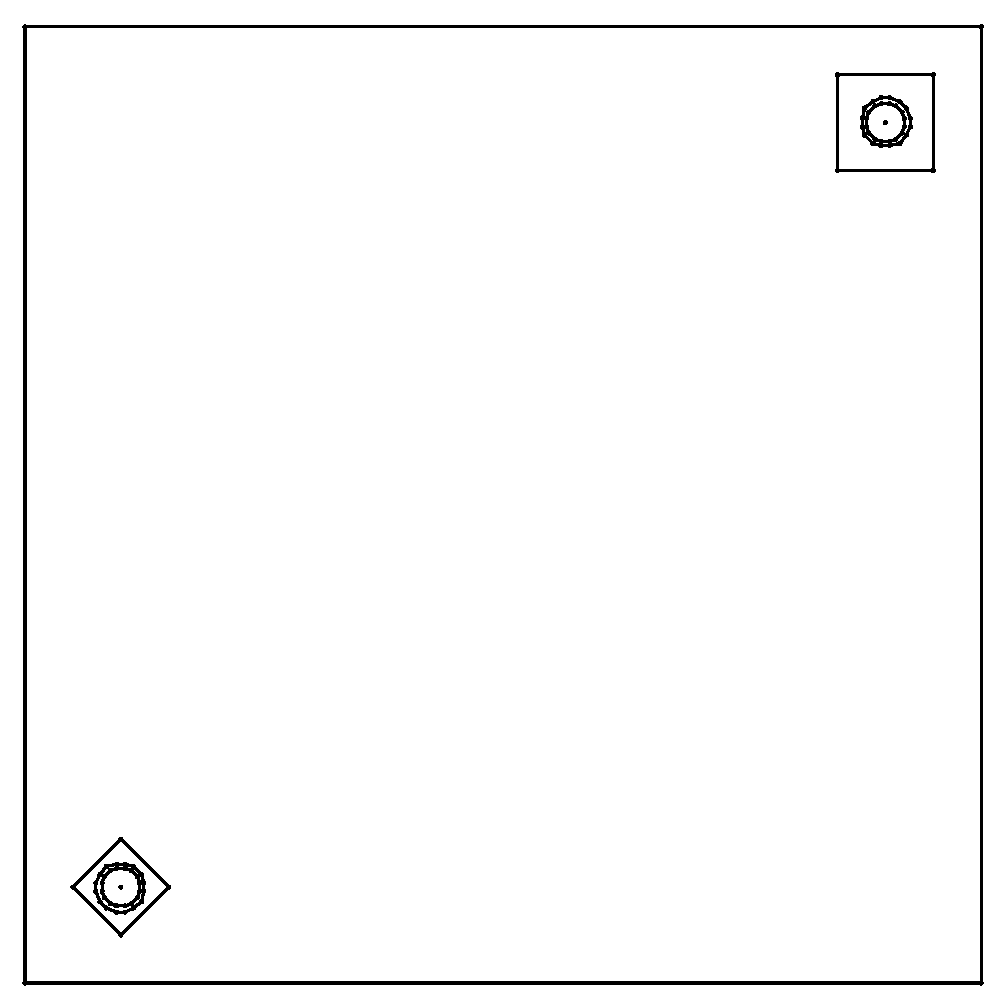
\includegraphics[scale = 0.5]{figures/unbalanced_lattice.eps}
\captionof{figure}{The first test case used in order to test effectiveness and convergence of the load balancing metric.}
\label{opp}
\end{minipage}

\noindent\begin{minipage}{\textwidth}
\centering
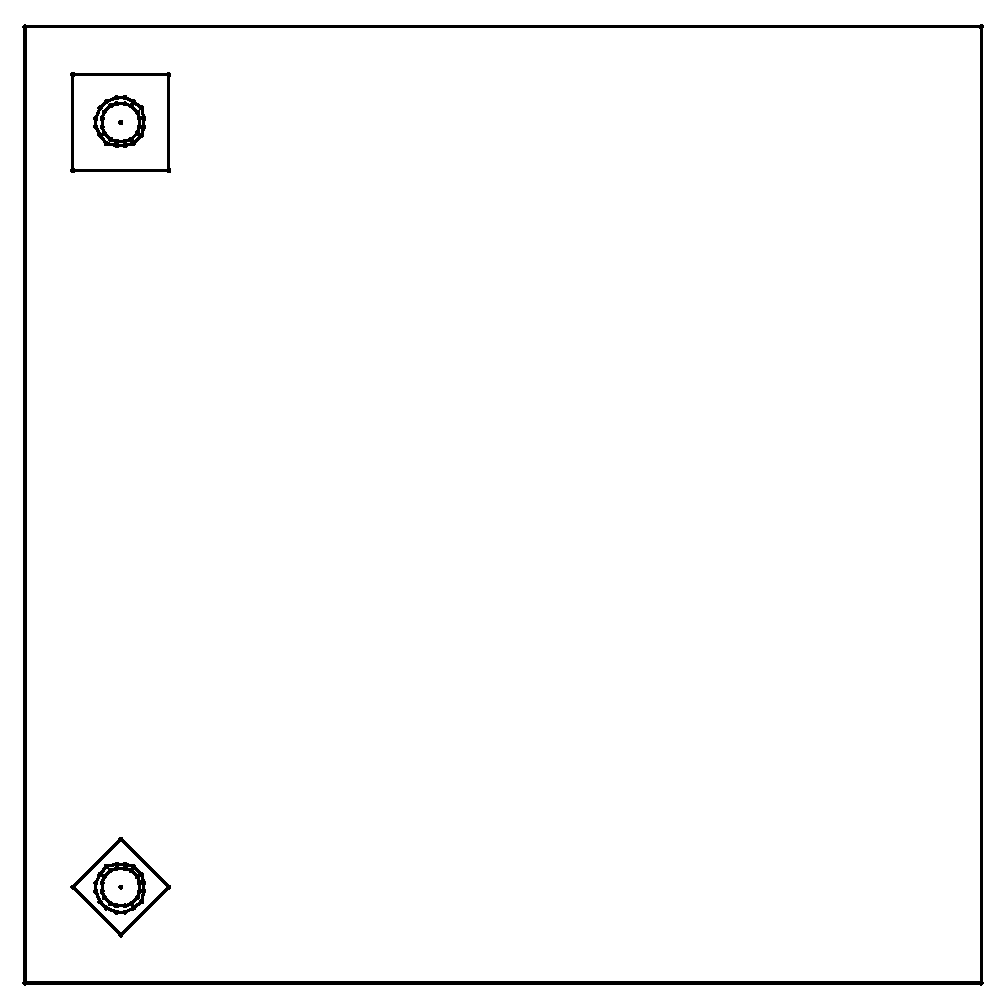
\includegraphics[scale = 0.5]{figures/unbalanced_pins_same_side.eps}
\captionof{figure}{The second test case used in order to test effectiveness and convergence of the load balancing metric.}
\label{same}
\end{minipage}


\noindent\begin{minipage}{\textwidth}
\centering
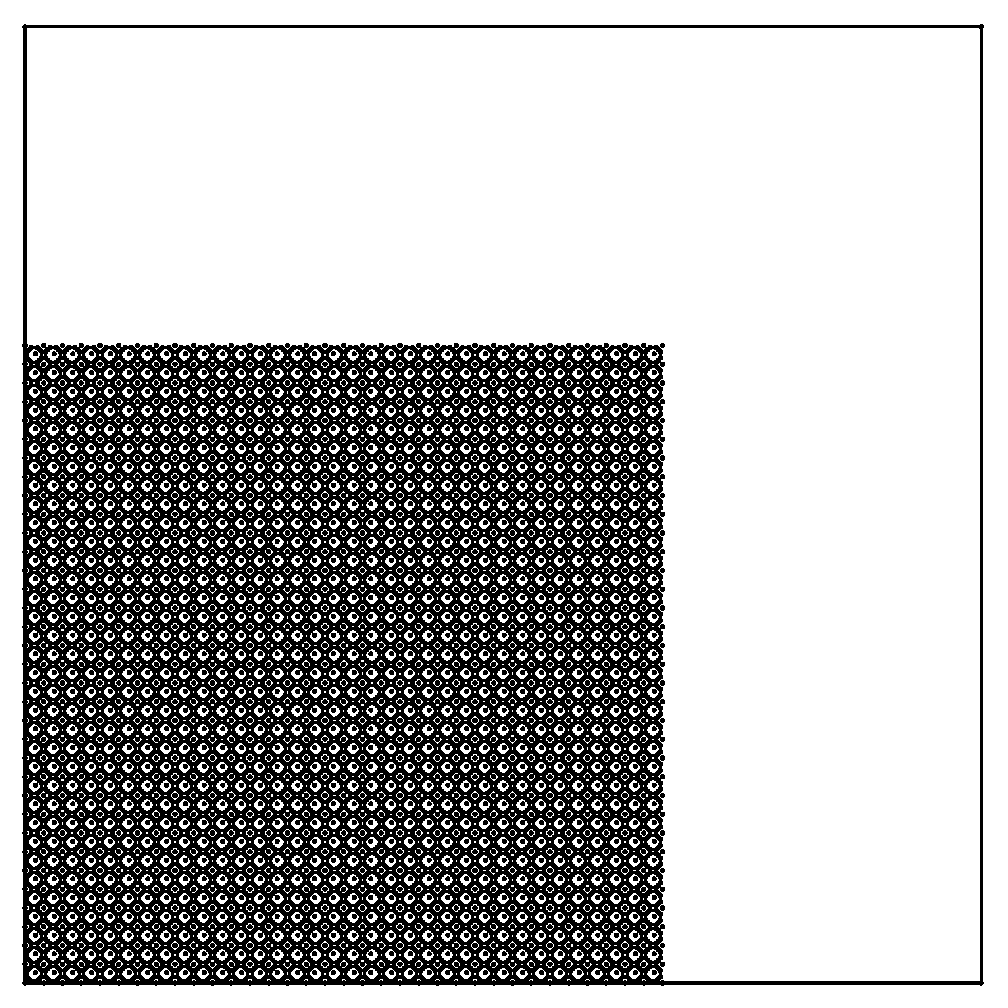
\includegraphics[scale = 0.5]{figures/lattice-12-shifted.eps}
\captionof{figure}{The third test case used in order to test effectiveness and convergence of the load balancing metric.}
\label{lattice}
\end{minipage}

\section{Metric Behavior and Convergence}

For each test case, the 162 input inputs are run twice, once with no load balancing iterations, and once with ten load balancing iterations. The best metric is reported and recorded. Three figures for each test cases are presented below: the first figure will show the metric behavior for no iterations, the second figure will show the metric behavior for each input run with ten load balancing iterations, and the third figure will show a ratio of the ten iteration runs over the no iteration runs.

Figure \ref{oppnoiter} shows the metric behavior for Fig. \ref{opp}. The maximum metric value is 24.7650, and occurs when Fig. \ref{opp} is run with 8x8 subsets and a maximum triangle area of 1.6 cm\textsuperscript{2}. The minimum metric value is 1.0016 and occurs when Fig. \ref{opp} is run with 4x4 subsets and a maximum triangle area of 0.04 cm\textsuperscript{2}. 

\noindent\begin{minipage}{\textwidth}
\centering
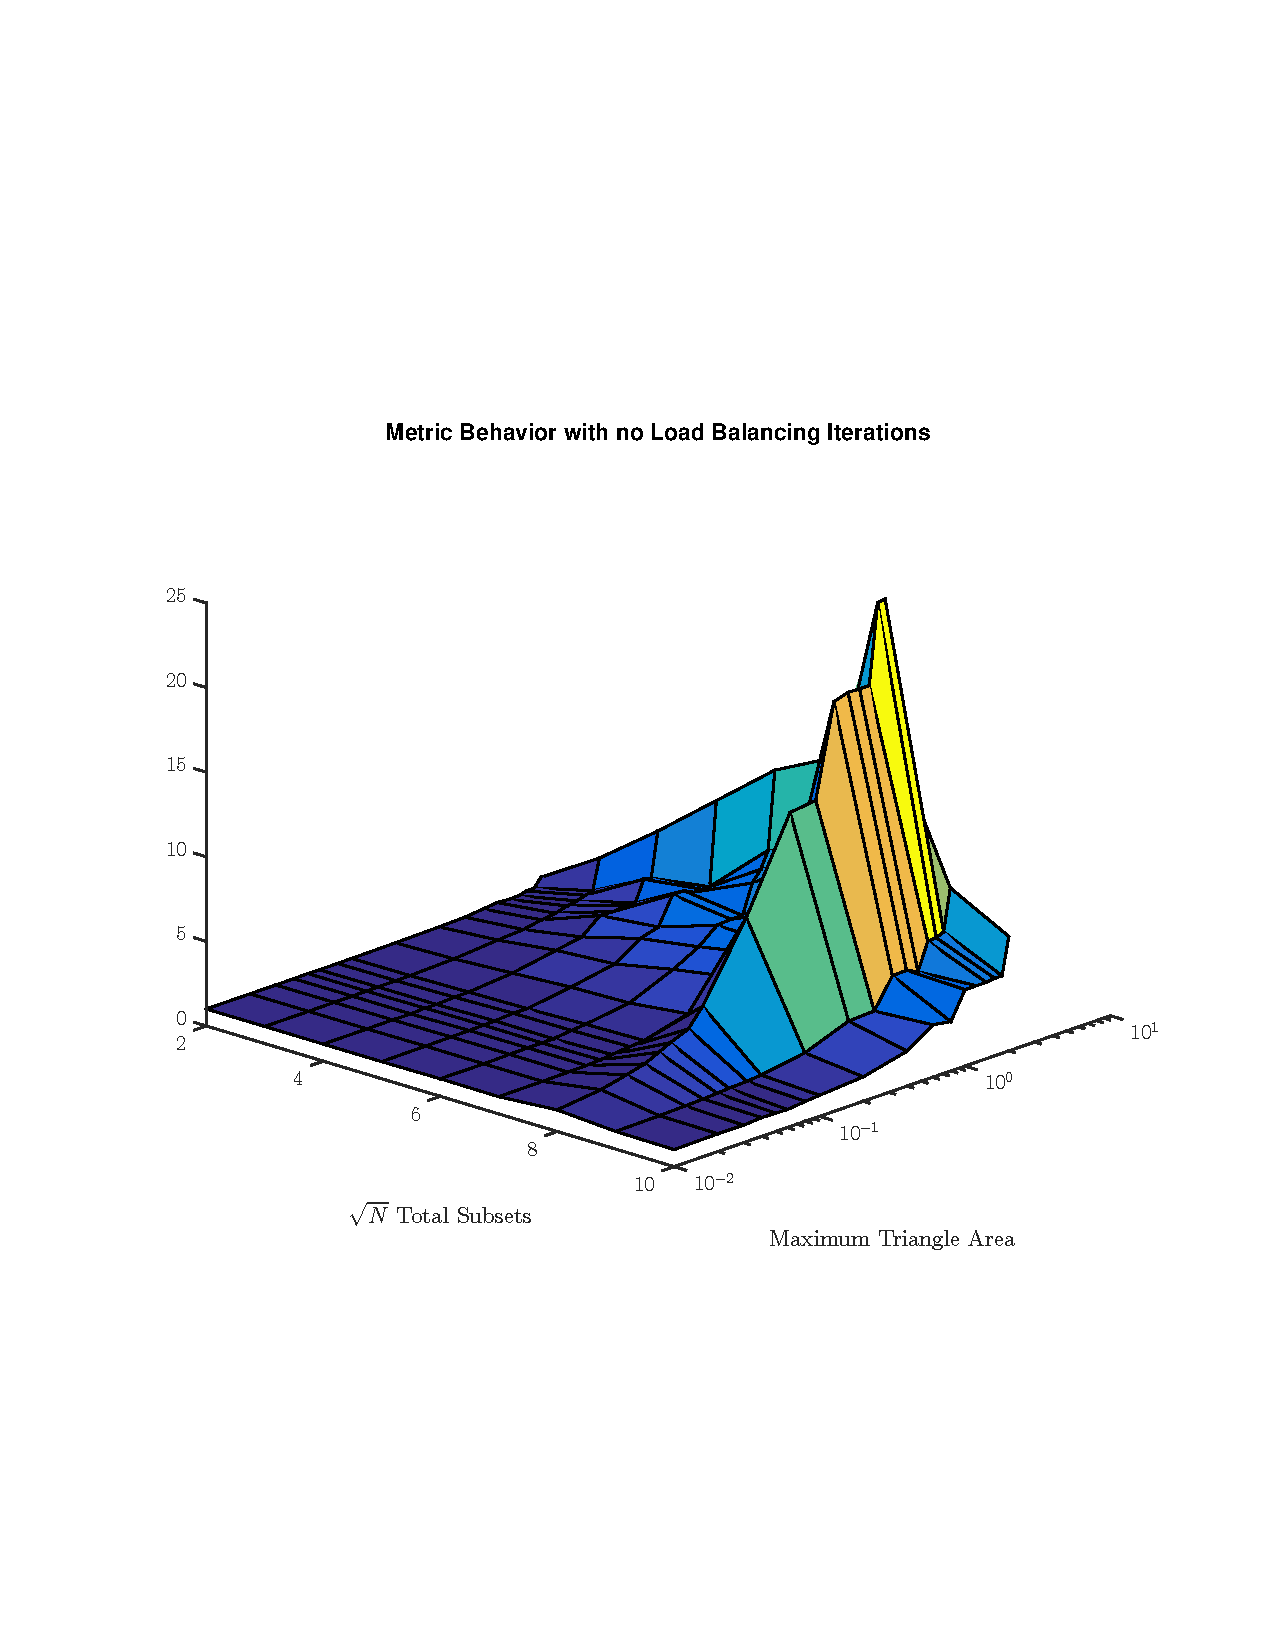
\includegraphics[scale=0.75, trim = 0cm 8cm 0cm 7cm,clip]{figures/OppNoIter.pdf}
\captionof{figure}{The metric behavior of the first test case run with no load balancing iterations.}
\label{oppnoiter}
\end{minipage}
\smallskip

Figure \ref{oppiter} shows the metric behavior for Fig. \ref{opp} after 10 load balancing iterations. The maximum metric value is 5.0538 and occurs when Fig. \ref{opp} is run with 10x10 subsets and a maximum triangle area of 1.2 cm\textsuperscript{2}. The minimum metric value is 1.0017 and occurs when Fig. \ref{opp} is run with 4x4 subsets and a maximum triangle area of 0.04 cm\textsuperscript{2}.

\noindent\begin{minipage}{\textwidth}
\centering
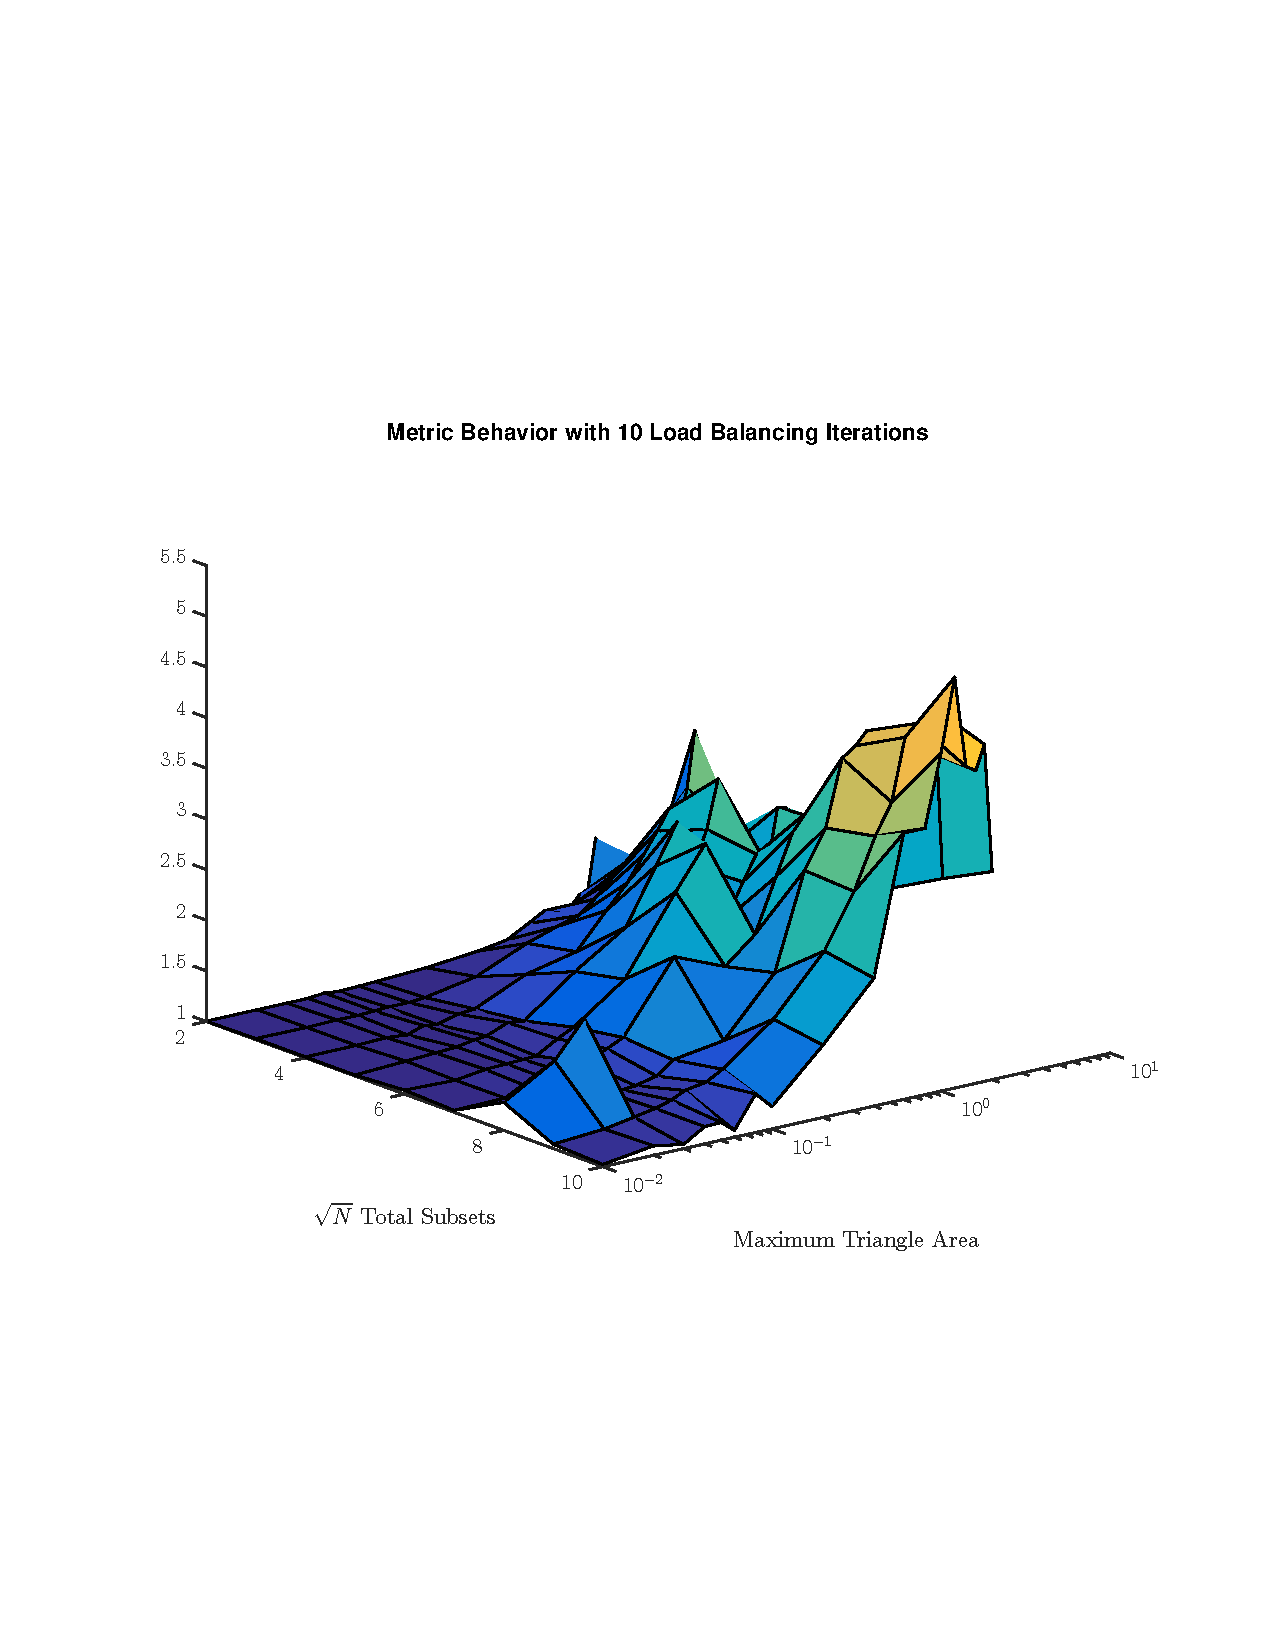
\includegraphics[scale=0.83, , trim = 2cm 6cm 2cm 7cm,clip]{figures/OppIter.pdf}
\captionof{figure}{The metric behavior of the first test case run with 10 load balancing iterations.}
\label{oppiter}
\end{minipage}
\smallskip

Figure \ref{oppdiff} shows the difference in metric behavior for Fig. \ref{opp}. This difference is calculated by dividing the metric with no iterations by the metric with 10 iterations. The maximum improvement has a value of 0.1097 and occurs for Fig. \ref{opp} is run with 8x8 subsets with a maximum triangle area of 1.6 cm\textsuperscript{2}. The minimum improvement has a value of very close to 1.0 and occurs for many of the inputs. 

\noindent\begin{minipage}{\textwidth}
\centering
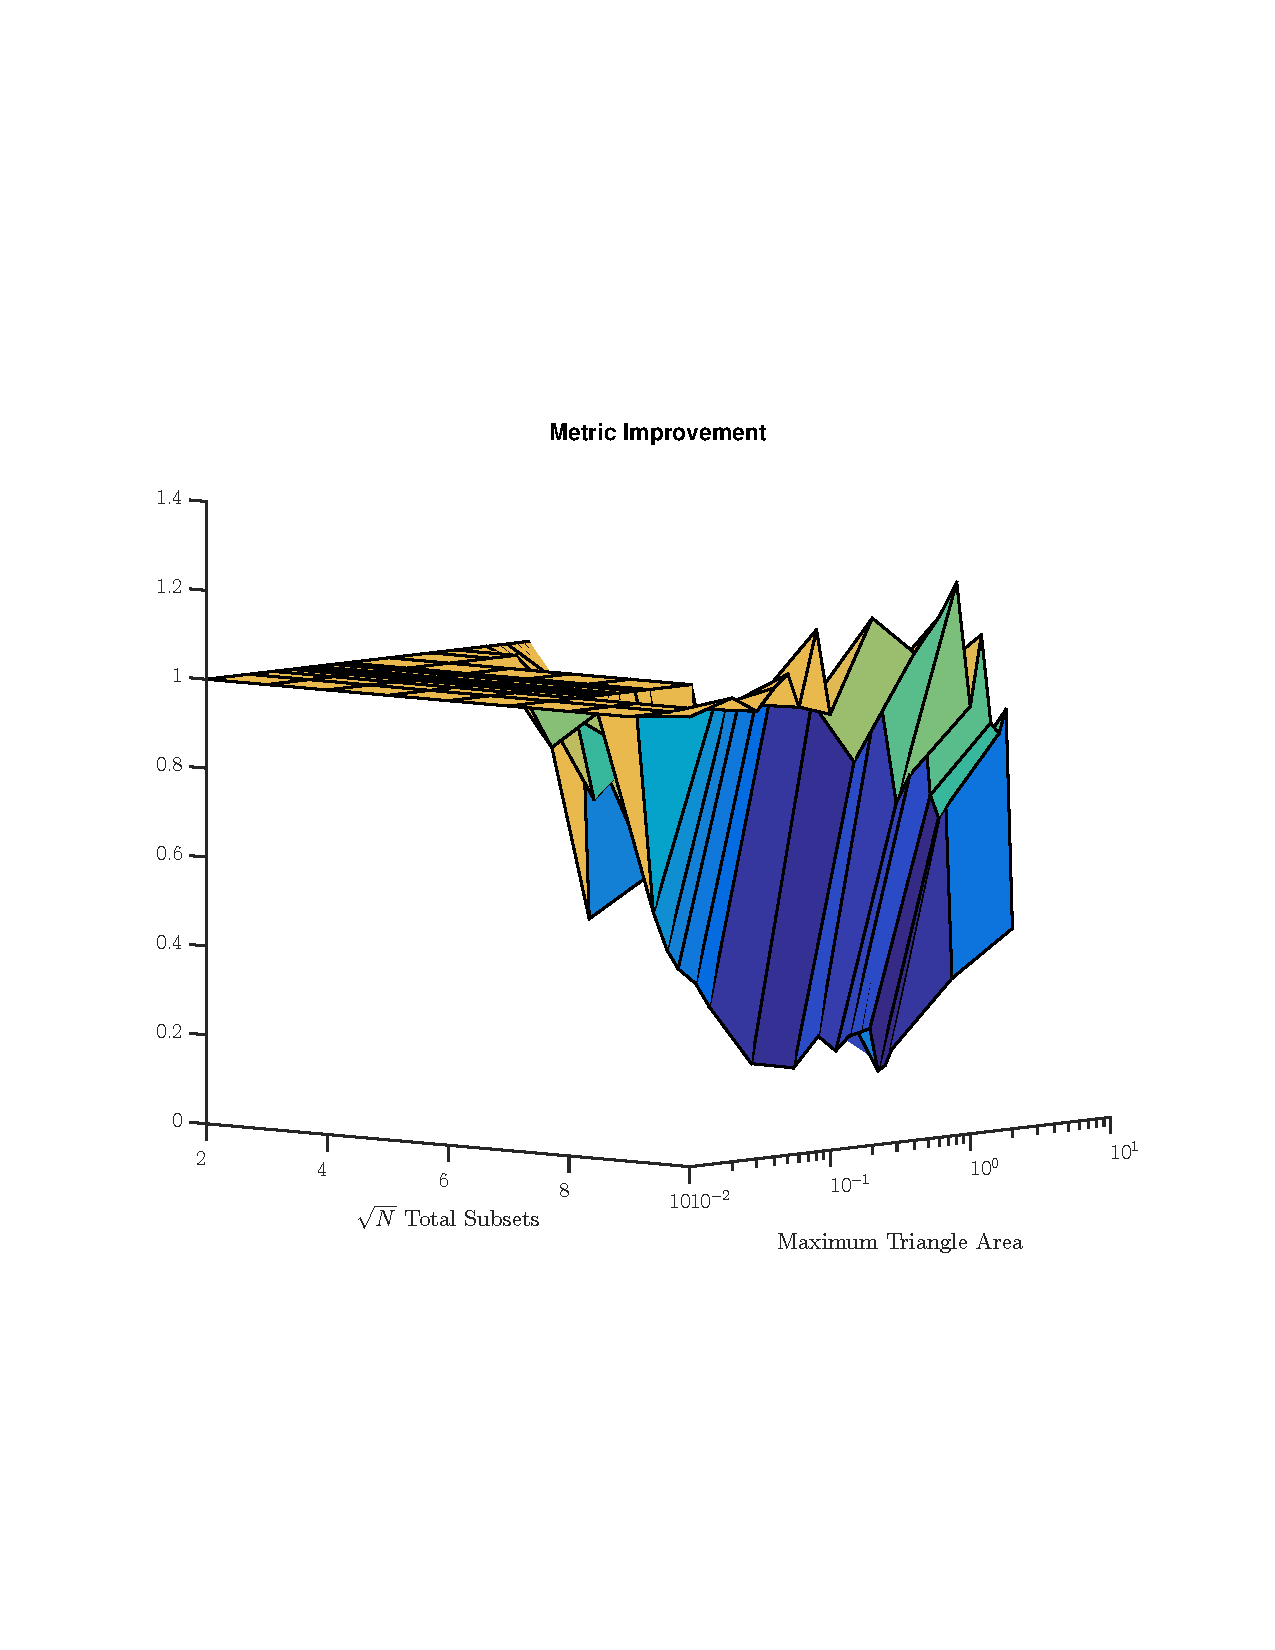
\includegraphics[scale=0.78, trim = 2cm 6cm 2cm 7cm,clip]{figures/OppDiff.pdf}
\captionof{figure}{The difference in metric behavior between no iteration and 10 iterations. The closer the z-value to zero, the better the improvement.}
\label{oppdiff}
\end{minipage}
\smallskip

Figure \ref{samenoiter} shows the metric behavior for Fig. \ref{same}. The maximum metric is 22.6654 and occurs when Fig. \ref{same} is run with 8x8 subsets with a maximum triangle area of 1.8 cm\textsuperscript{2}. The minimum metric is 1.0024 and occurs when Fig. \ref{same} is run with 2x2 subsets with a maximum triangle are of 0.01 cm\textsuperscript{2}.

\noindent\begin{minipage}{\textwidth}
\centering
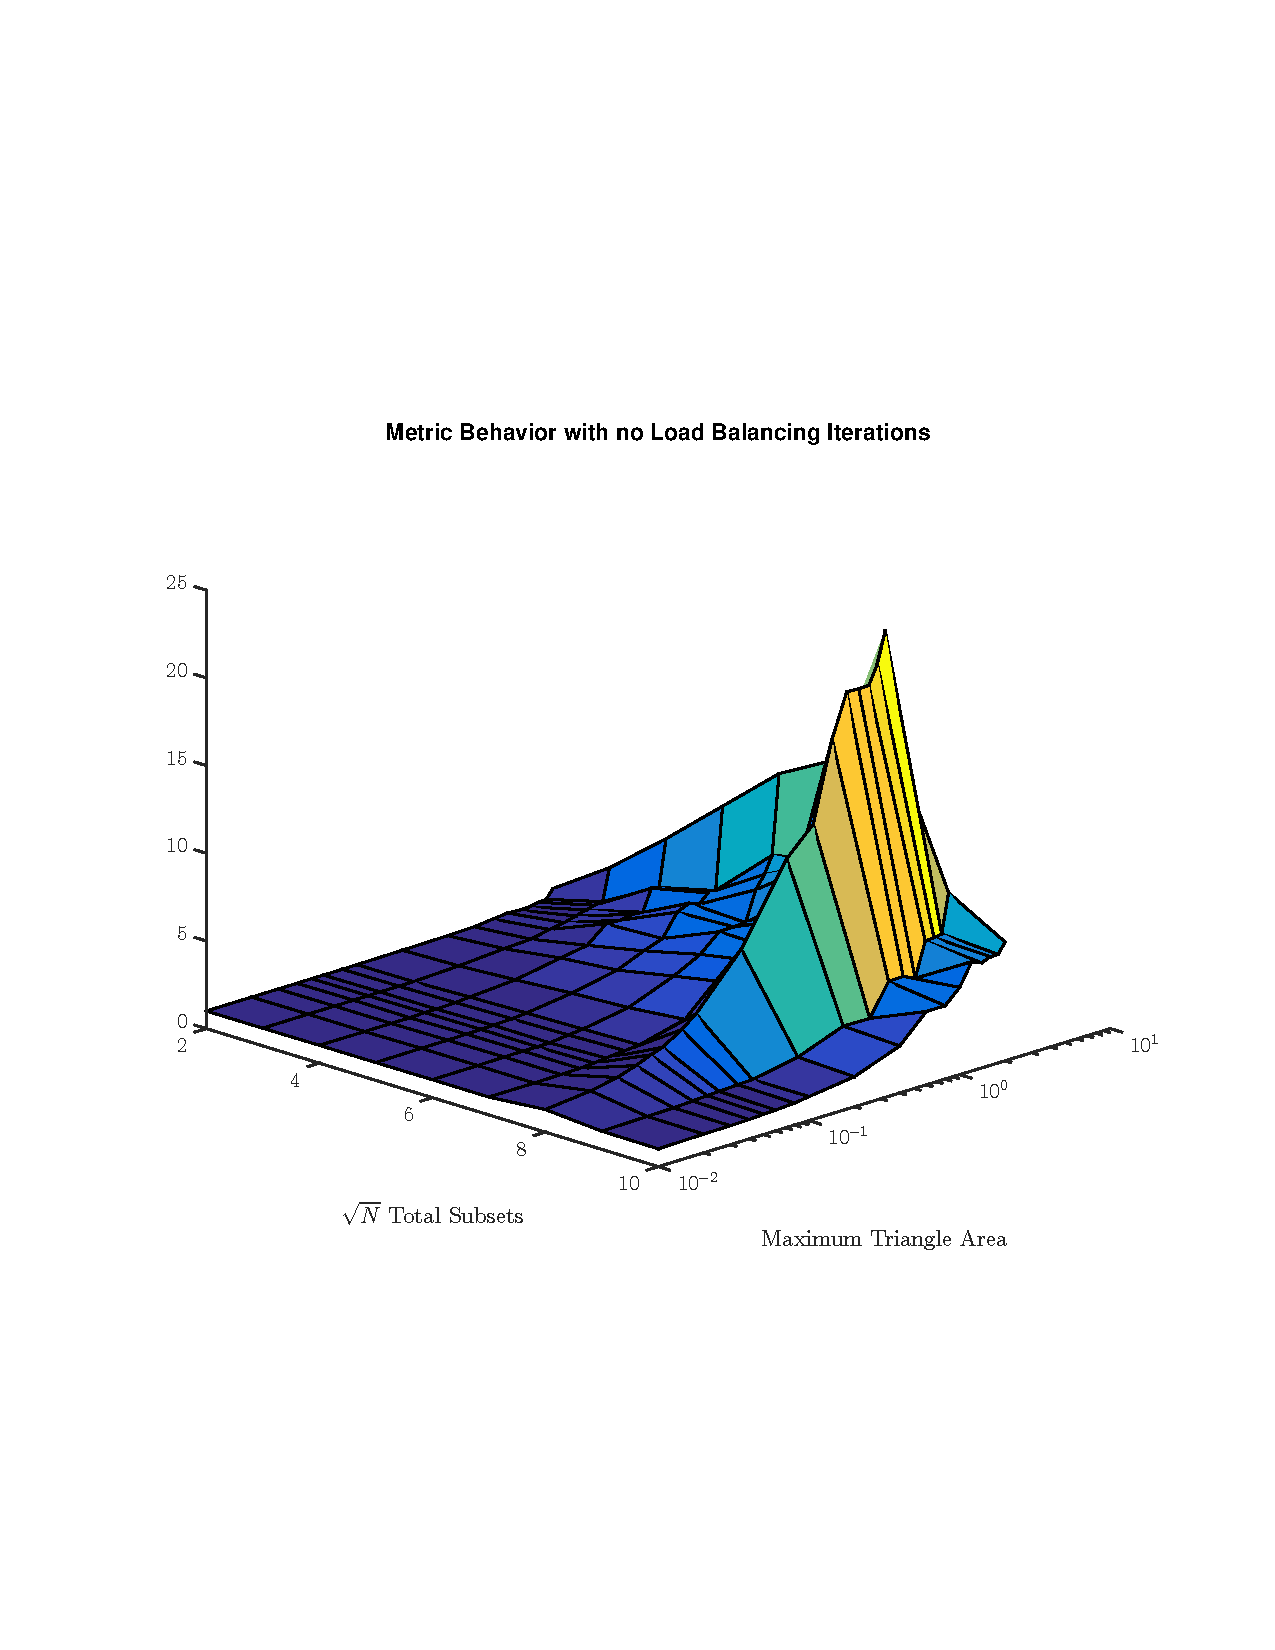
\includegraphics[scale=0.78, trim = 2cm 6cm 2cm 7cm,clip]{figures/SameNoIter.pdf}
\captionof{figure}{The metric behavior of the second test case run with no load balancing iterations.}
\label{samenoiter}
\end{minipage}
\smallskip

Figure \ref{sameiter} shows the metric behavior for Fig. \ref{same} after ten load balancing iterations. The maximum metric is 3.9929 and occurs when Fig. \ref{same} is run with 10x10 subsets with a maximum triangle area of 1.8 cm\textsuperscript{2}. The minimum metric is 1.0024 and occurs when Fig. \ref{same} is run with 2x2 subsets with a maximum triangle are of 0.01 cm\textsuperscript{2}.

\noindent\begin{minipage}{\textwidth}
\centering
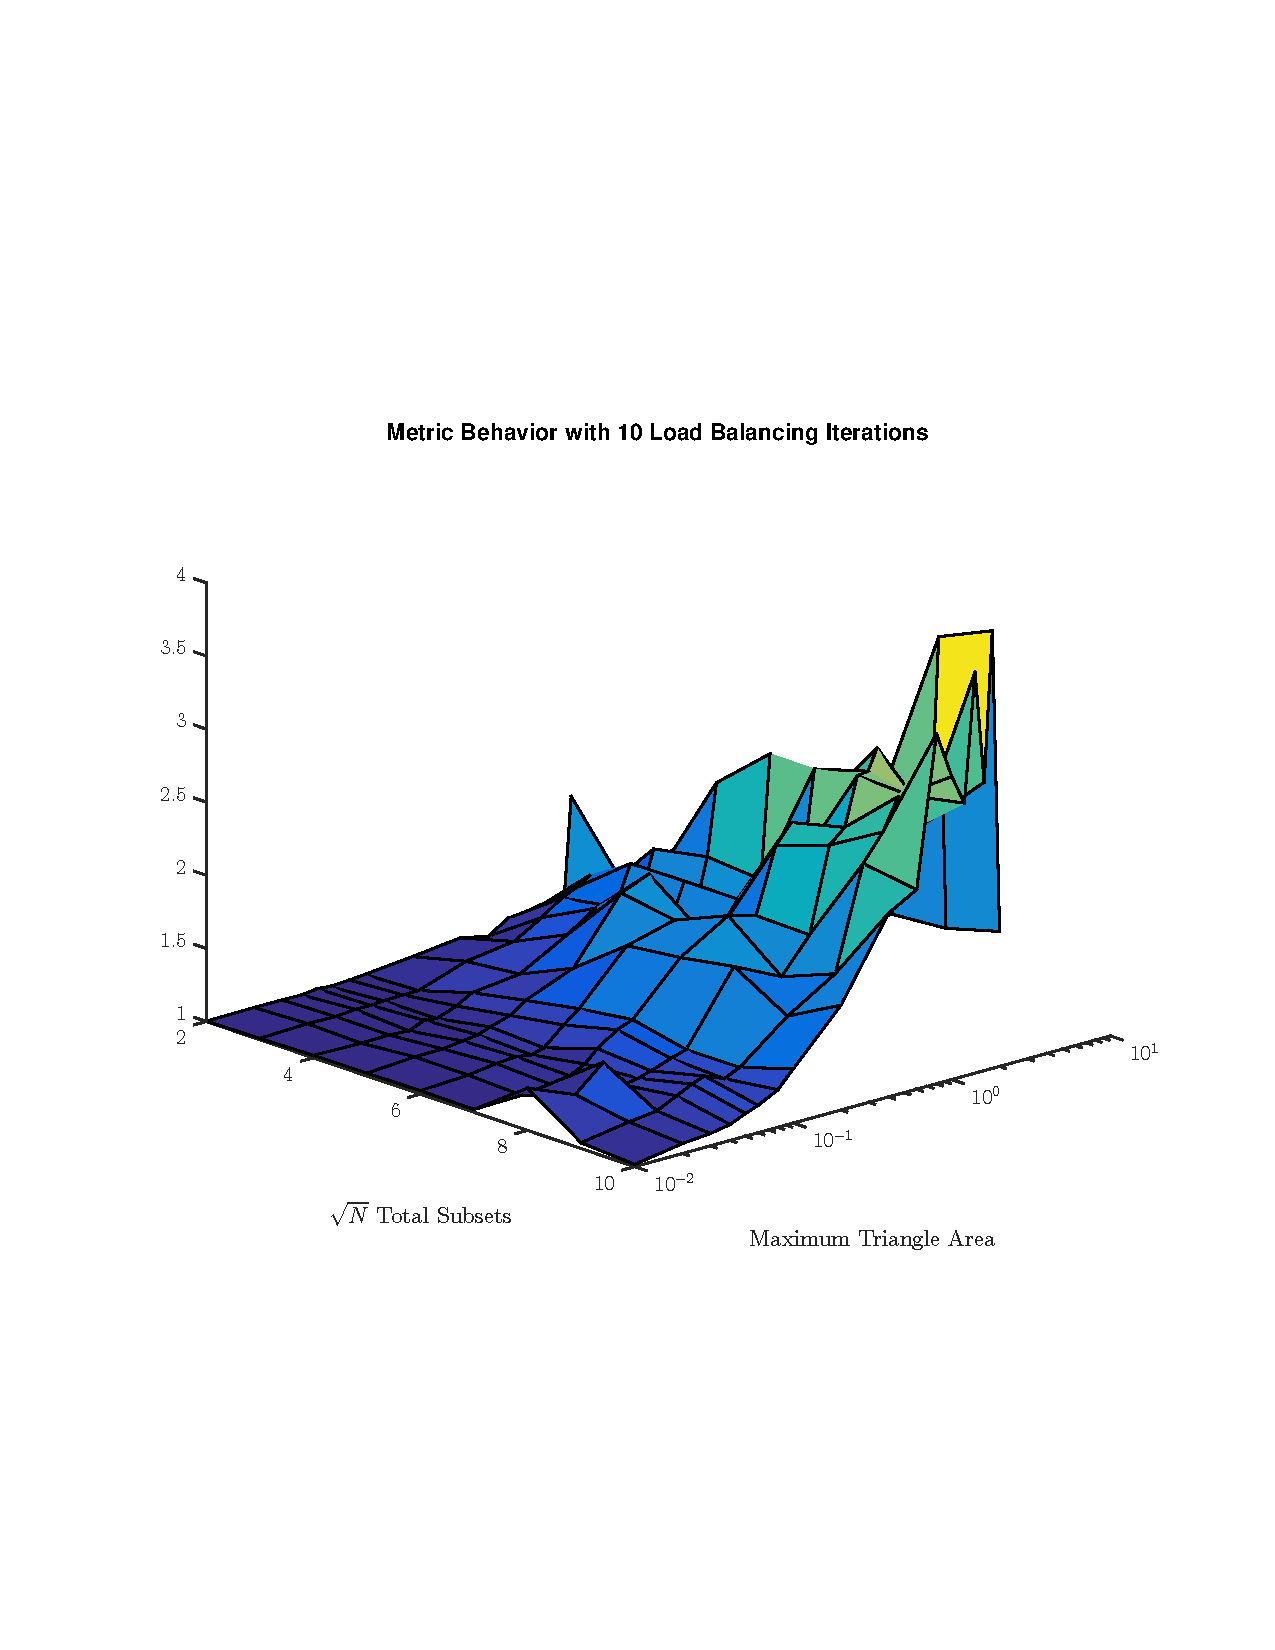
\includegraphics[scale=0.80, trim = 2cm 6cm 2cm 7cm,clip]{figures/SameIter.pdf}
\captionof{figure}{The metric behavior of the second test case run with 10 load balancing iterations.}
\label{sameiter}
\end{minipage}
\smallskip

Figure \ref{samediff} shows the difference in metric behavior for Fig. \ref{same}. The maximum improvement has a value of 0.1090 and occurs for Fig. \ref{same} is run with 8x8 subsets with Triangle's coarsest possible mesh generation settings. The minimum improvement has a value of very close to 1.0 and occurs for many of the inputs. 

\noindent\begin{minipage}{\textwidth}
\centering
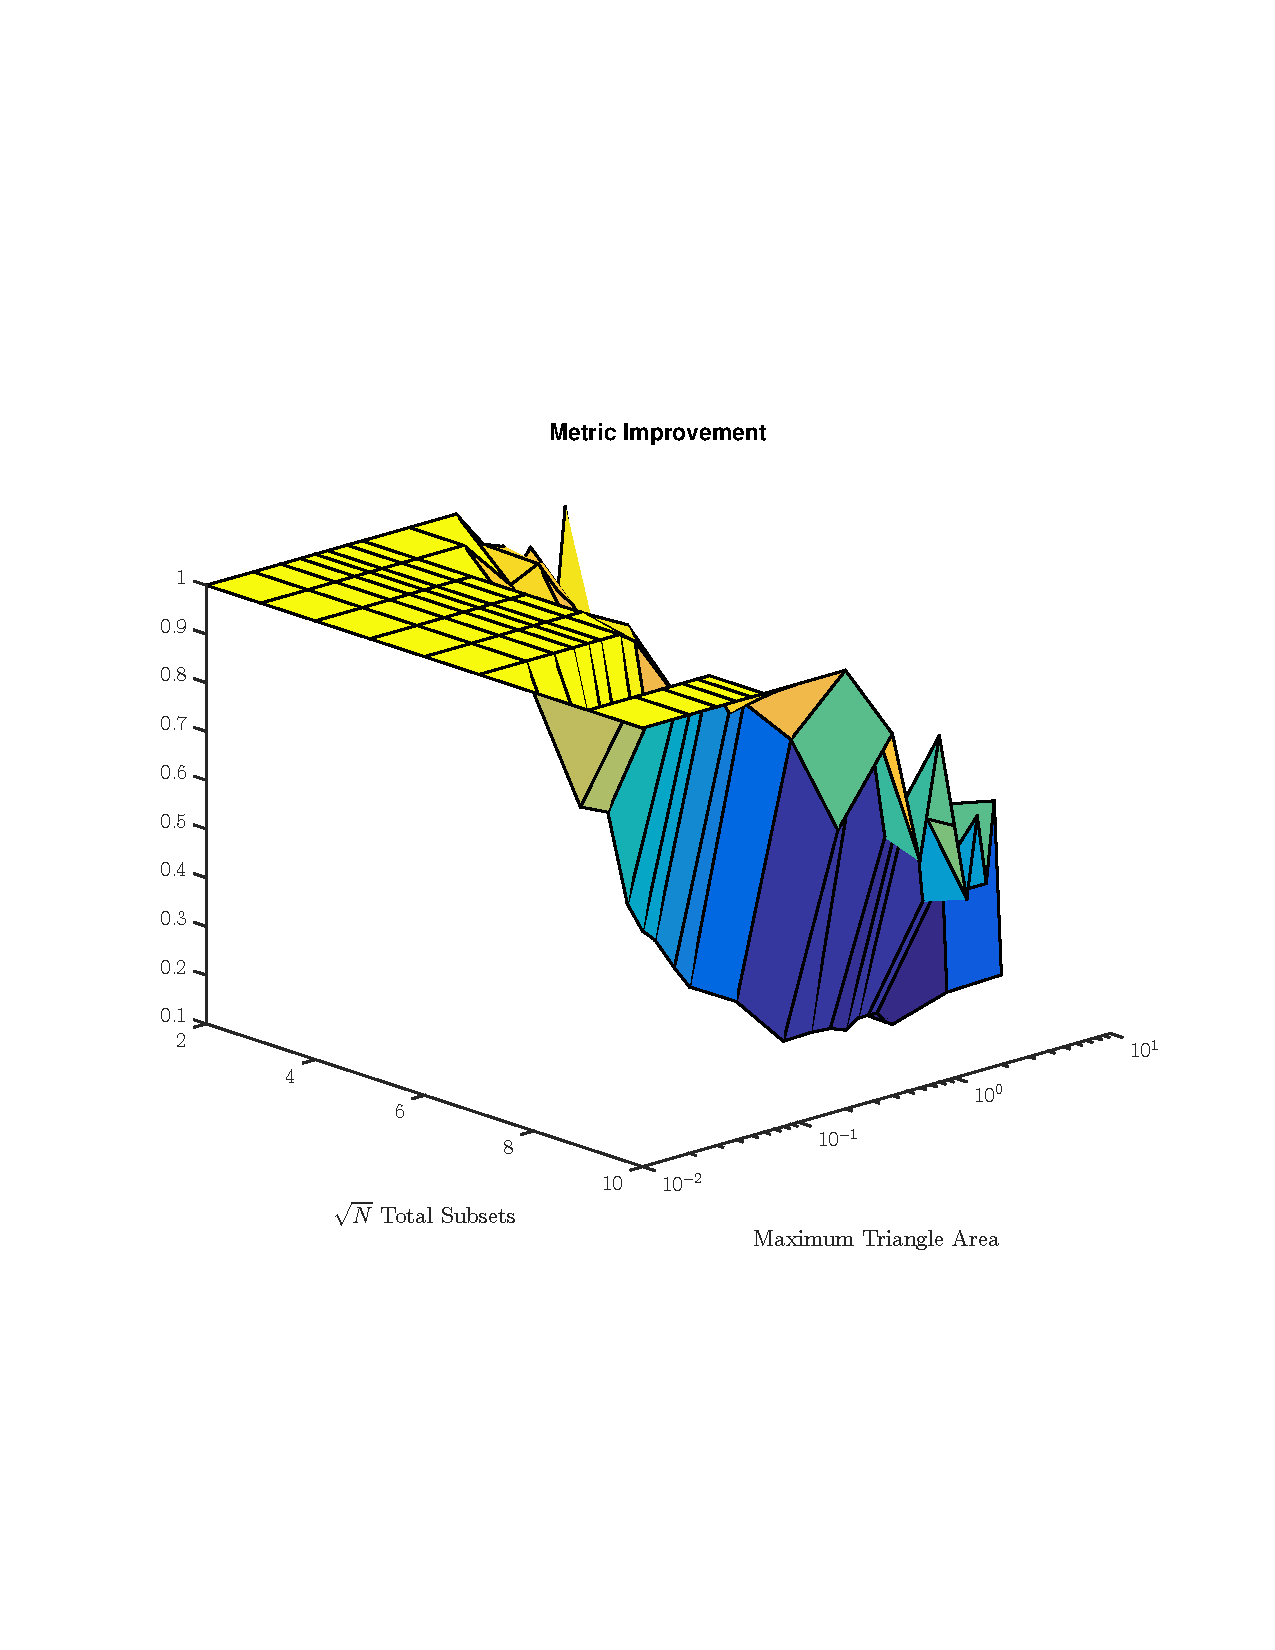
\includegraphics[scale=0.80, trim = 2cm 6cm 2cm 7cm,clip]{figures/SameDiff.pdf}
\captionof{figure}{The difference in metric behavior of the second test case with no iteration and 10 iterations. The closer the z-value to zero, the better the improvement.}
\label{samediff}
\end{minipage}
\smallskip

Figure \ref{latticenoiter} shows the metric behavior for Fig. \ref{lattice}. The maximum metric is 2.6489 and occurs when Fig. \ref{lattice} is run with 10x10 subsets with a maximum triangle area of 1.8 cm\textsuperscript{2}. The minimum metric is 1.0179 and occurs when Fig. \ref{lattice} is run with 2x2 subsets with a maximum triangle are of 0.08 cm\textsuperscript{2}.

\noindent\begin{minipage}{\textwidth}
\centering
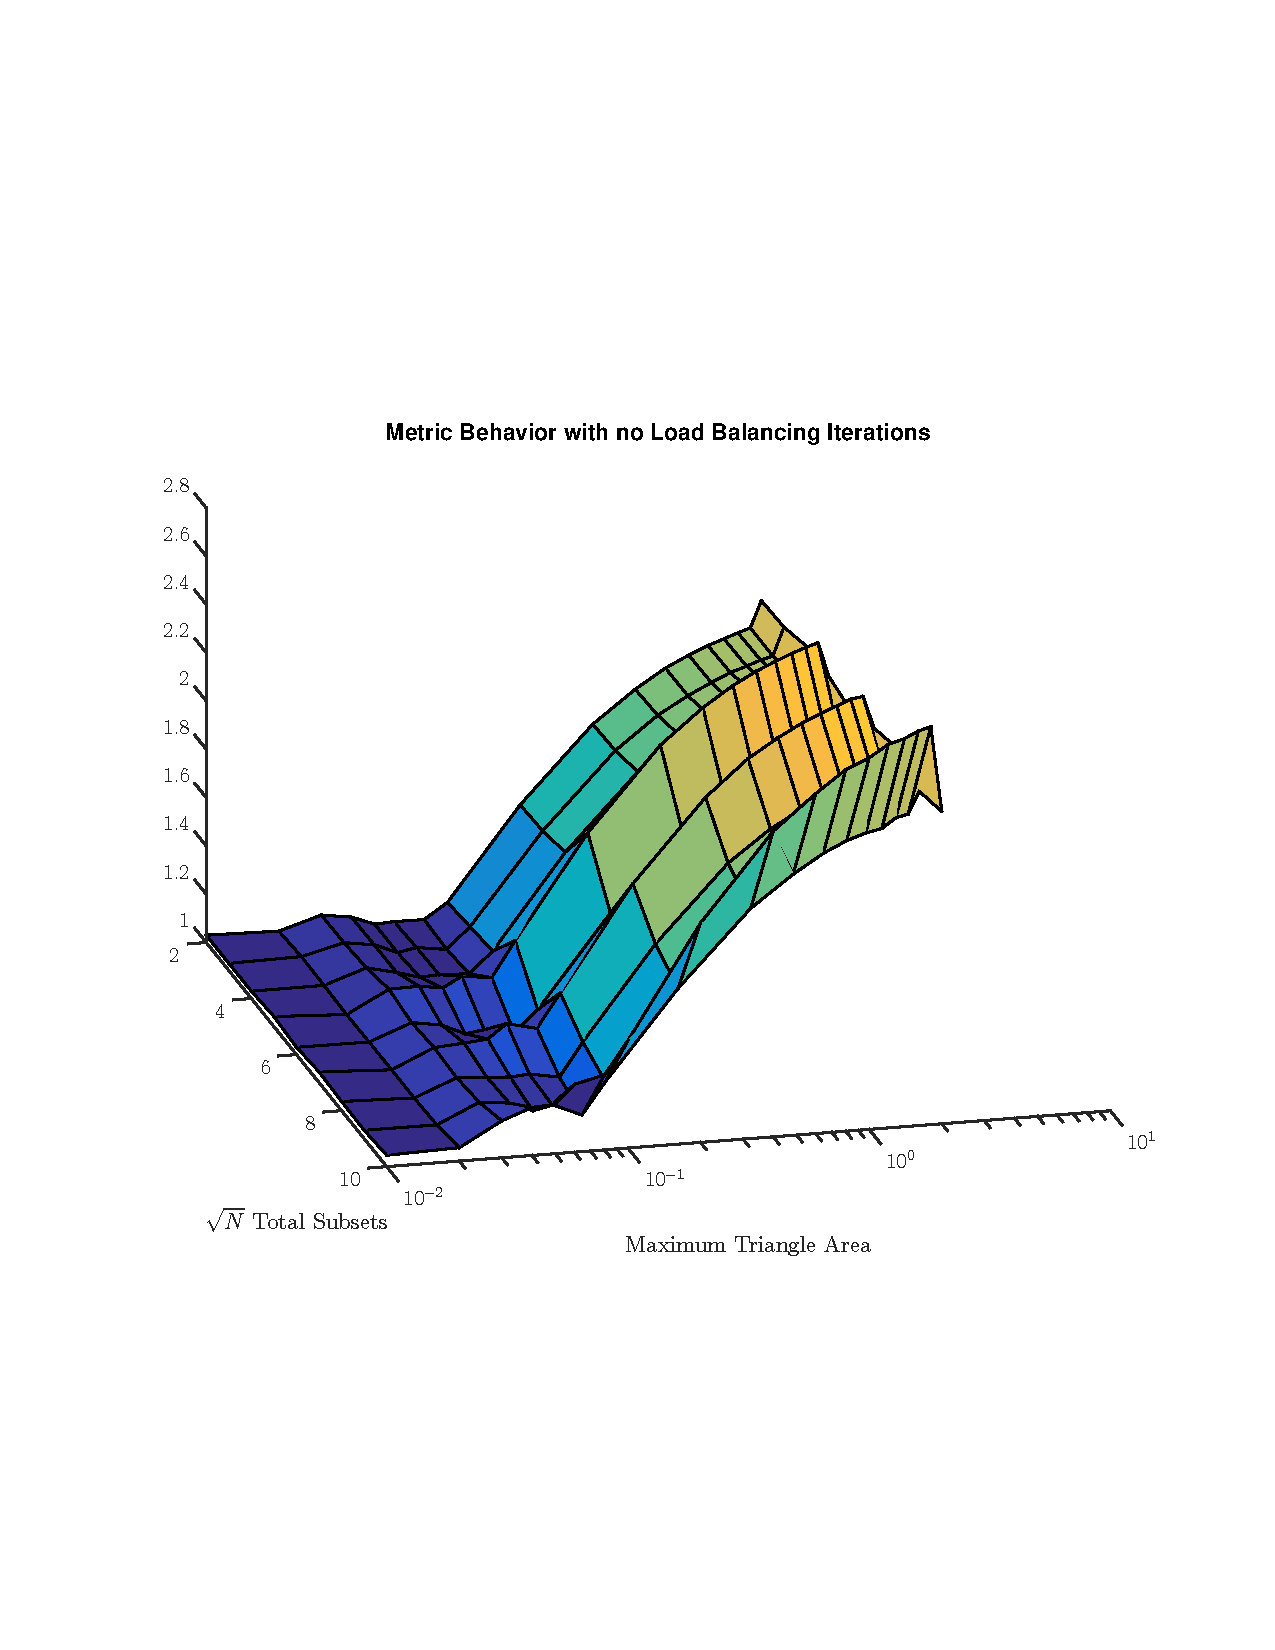
\includegraphics[scale=0.80, trim = 2cm 6cm 2cm 7cm,clip]{figures/lattice_no_iter.pdf}
\captionof{figure}{The difference in metric behavior of the third test case with no load balancing iterations.}
\label{latticenoiter}
\end{minipage}
\smallskip

Figure \ref{latticeiter} shows the metric behavior for Fig. \ref{lattice} after ten load balancing iterations. The maximum metric is 2.2660 and occurs when Fig. \ref{lattice} is run with 10x10 subsets with a maximum triangle area of 0.4 cm\textsuperscript{2}. The minimum metric is 1.0021 and occurs when Fig. \ref{lattice} is run with 2x2 subsets with the Triangle's coarsest possible mesh.

\noindent\begin{minipage}{\textwidth}
\centering
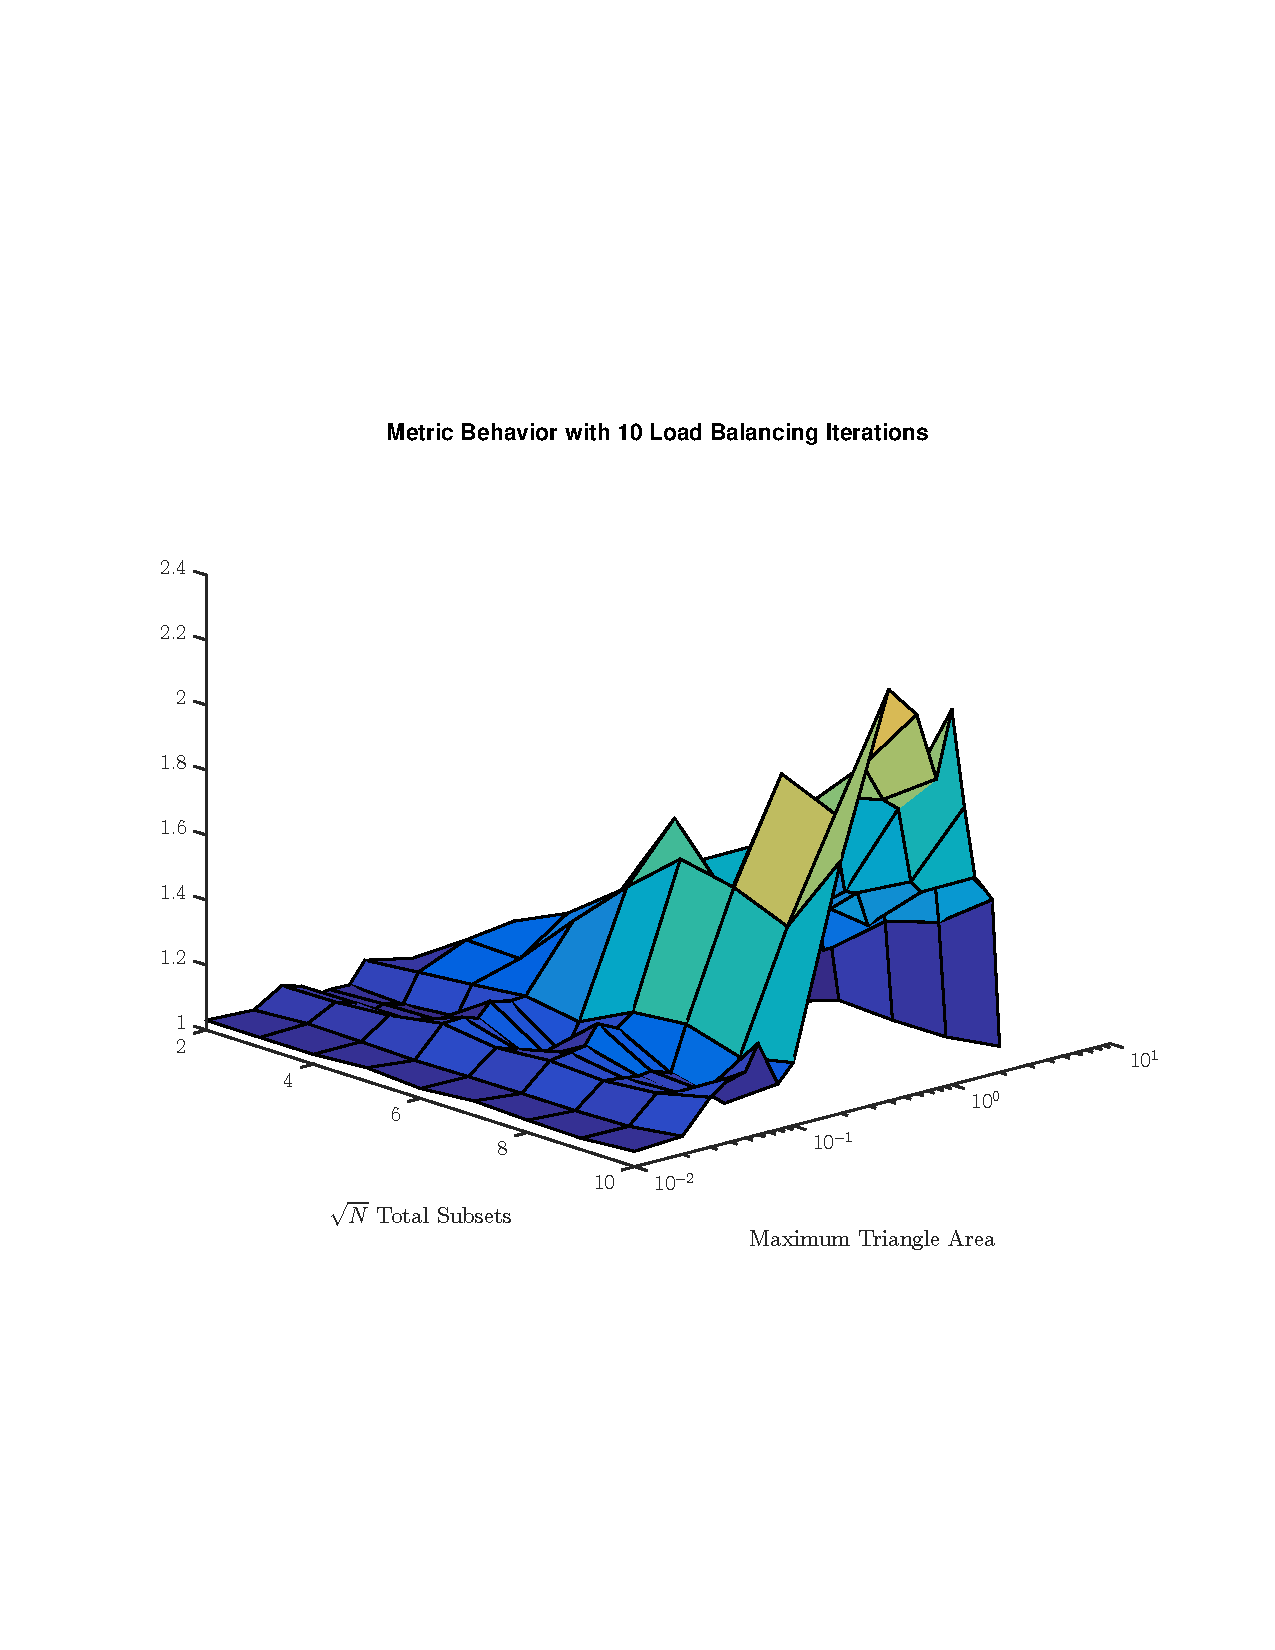
\includegraphics[scale=0.80, trim = 2cm 6cm 2cm 7cm,clip]{figures/lattice_iter.pdf}
\captionof{figure}{The difference in metric behavior of the third test case after ten load balancing iterations.}
\label{latticeiter}
\end{minipage}
\smallskip

Figure \ref{latticediff} shows the difference in metric behavior for Fig. \ref{lattice}. The maximum improvement has a value of 0.4476 and occurs for Fig. \ref{lattice} is run with 2x2 subsets with Triangle's coarsest possible mesh generation settings. The minimum improvement has a value of very close to 1.0 and occurs for many of the inputs. 

\noindent\begin{minipage}{\textwidth}
\centering
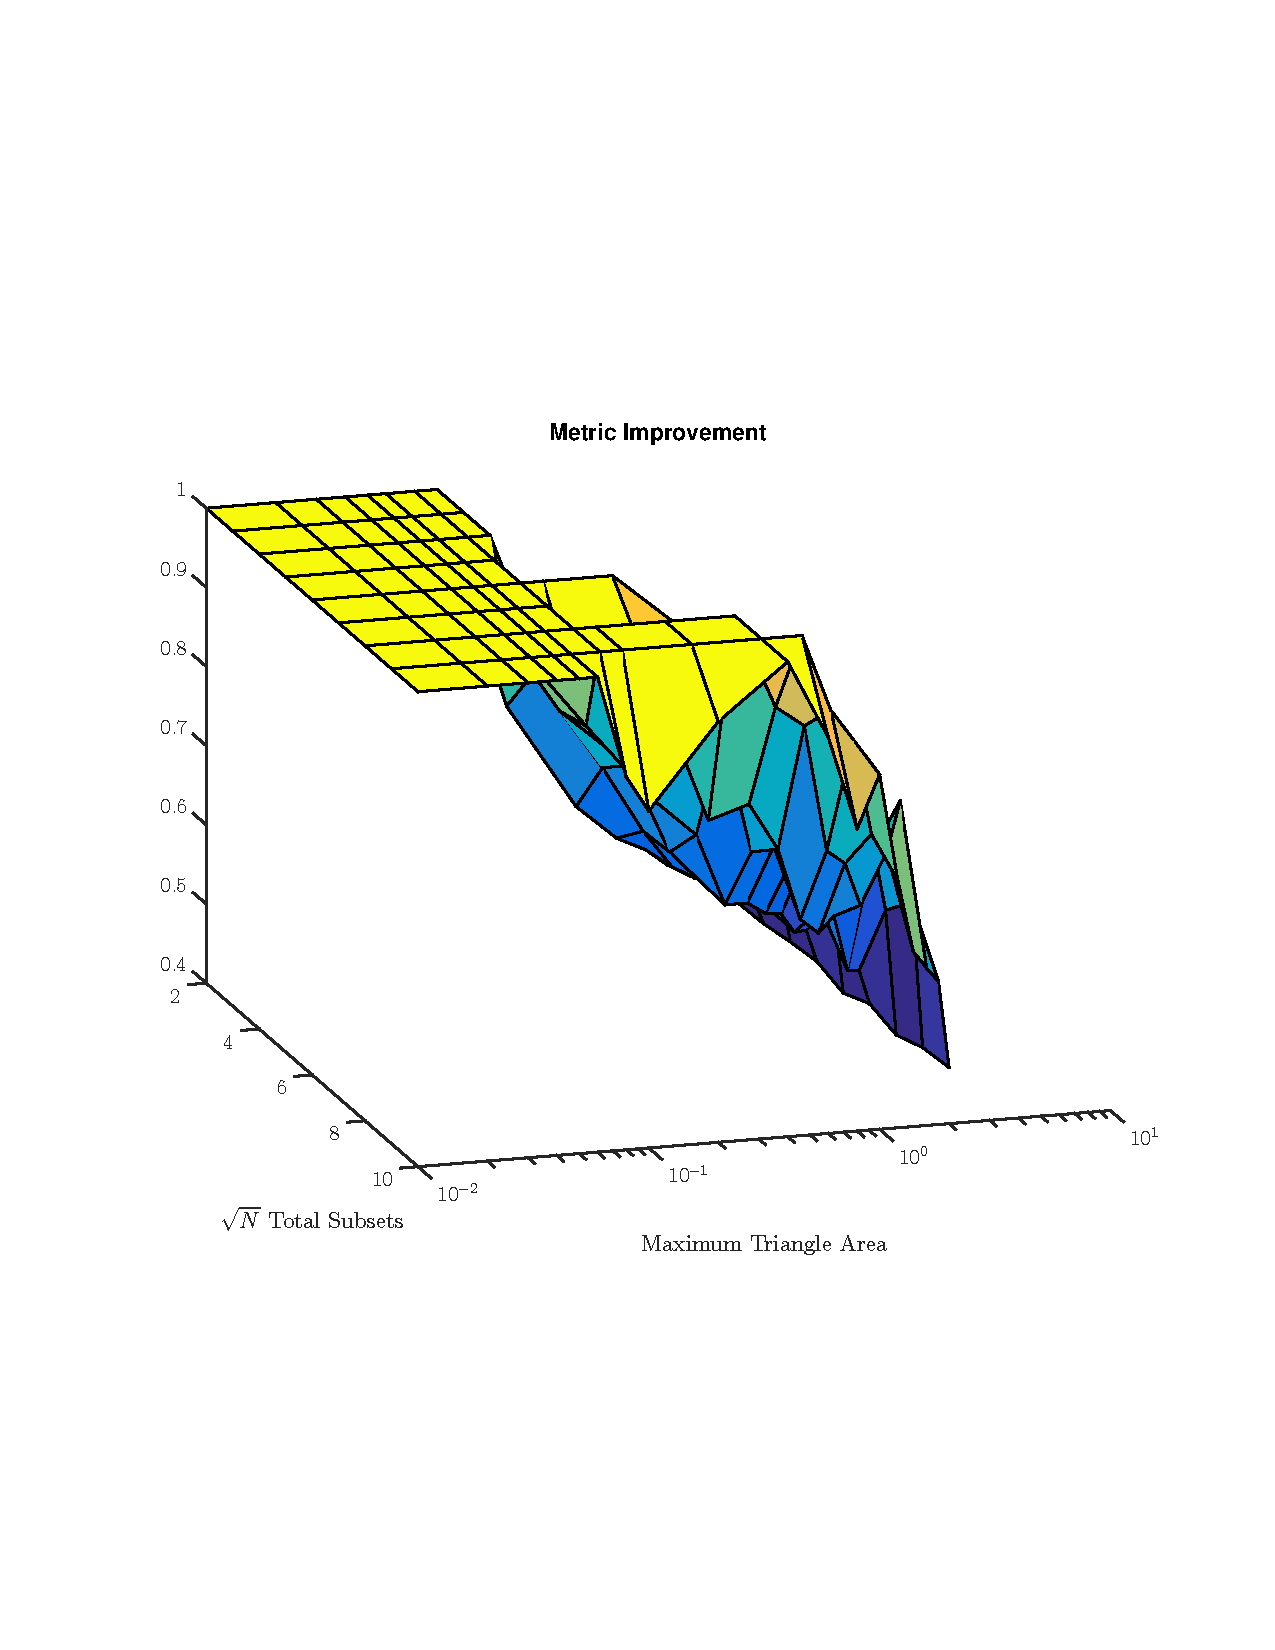
\includegraphics[scale=0.80, trim = 2cm 6cm 2cm 7cm,clip]{figures/lattice_diff.pdf}
\captionof{figure}{The difference in metric behavior of the third test case with no iteration and 10 iterations. The closer the z-value to zero, the better the improvement.}
\label{latticediff}
\end{minipage}
\smallskip

Because Fig. \ref{lattice} has more features and is more symmetric of a problem, the initial load balancing metric will not be as large as the load balancing metric of Figs. \ref{same} and \ref{opp}. As a result, the improvement in the load balancing metric after 10 iterations will not be as great in problems similar to Fig. \ref{lattice}. 

Good improvement is seen throughout all three test cases for all three inputs, particularly the first two test cases, which were initially very unbalanced. However, there were many inputs run that had problems with $f > 1.1$, which means many problems were unbalanced by more than 10\%. The user will not always have the luxury of choosing the number of subsets they want the problem run with, as this directly affects the number of processors the problem will be run with. Certain problems will require more processors and will require minimizing the total number of cells in the domain for the problem to complete running in a reasonable amount of time. As a result, improvements to the algorithm must be made. 

This can be done by changing how the cut lines are redistributed. Instead of changing entire row and column widths, the cut lines can be moved on the subset level. However, this can sacrifice the strict orthogonality that PDT currently utilizes to scale so well on a massively parallel scale. Changes to the performance model and the scheduler would have to be made.

Another option is to implement domain overloading, which is the logical extension of the work presented in this thesis. This would involve processors owning different numbers of subsets, with no restriction on these subsets being contiguous. This would be the most effective method at perfecting this algorithm, and would lead to less problems being unbalanced by more than 10\%.

\section{Solution Verification}

For solution verification, two simple problems were chosen: a 1D pure absorber slab and a 1D pure scatterer slab. These problems were chosen because their analytical solutions are easily obtained, thus making a comparison between PDT's solution and the analytical solution easy and informative. The same geometry and mesh were used for both problems, and are shown in Figure \ref{verificationgeometry}.

\noindent\begin{minipage}{\textwidth}
\centering
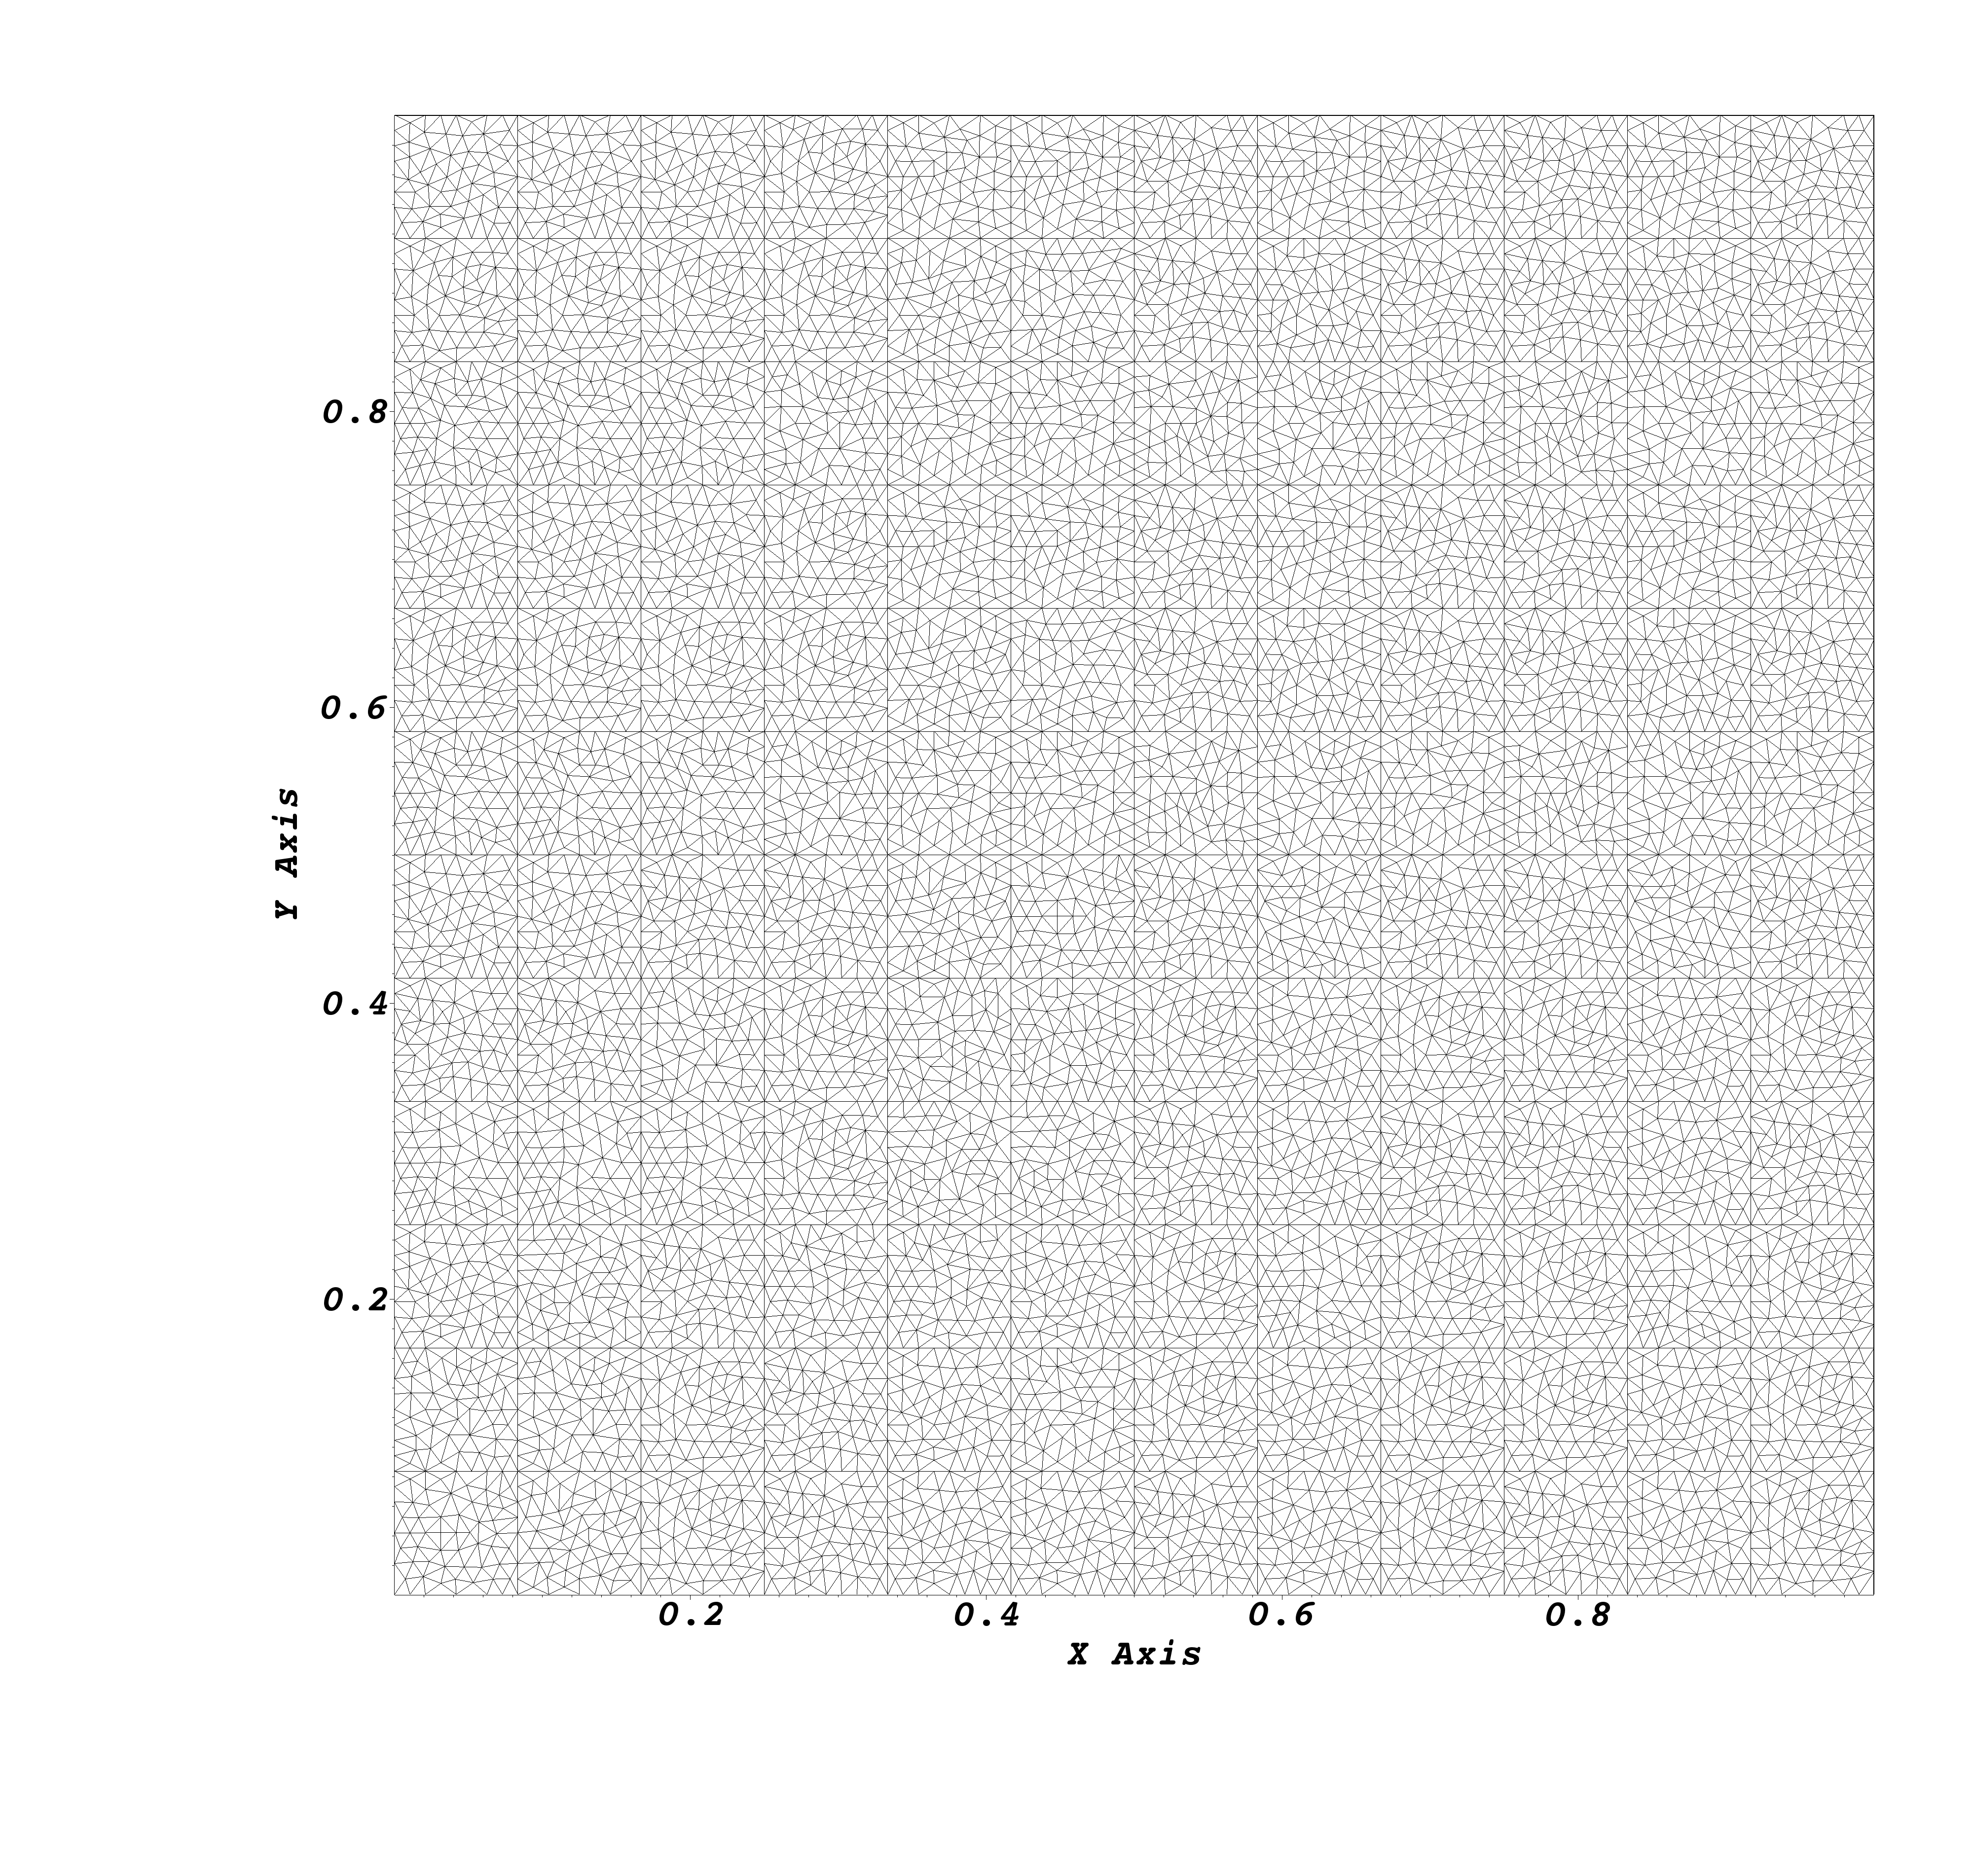
\includegraphics[scale = 0.12,trim = 10cm 10cm 0cm 0cm ]{figures/solutionmesh.png}
\captionof{figure}{The geometry and mesh used in solution verification problems.}
\label{verificationgeometry}
\end{minipage}
\smallskip

The problem geometry is a 1 cm by 1 cm square. In order to simulate a 1D slab, opposing reflecting boundaries were placed on the both y boundaries, effectively forcing the problem to be infinite in the y direction. At the x minimum boundary, an incident isotropic flux was used, and a vacuum boundary was enforced at the x max boundary. No source was used in either problem.

In order to measure how close the numerical and analytical solutions an error estimate, represented by, Eq. ~\eqref{error}, is used:
\begin{equation}
\epsilon = \sqrt{\sum_k \sum_q w_q \cdot(\phi_h(x_q) - \phi_e(x_q))^2}
%\epsilon = \frac{\norm{\text{Analytical} - \text{ Numerical}}_{l2}}{\norm{\text{Analytical}}_{l2}},
\label{error}
\end{equation}
where $k$ is the number of cells, $q$ is the number points per cell used in a Gauss-Legendre quadrature, $phi_h$ is the numerical flux solution and $phi_e$ is the analytical flux solution.

\subsection{The 1D Pure Absorber Slab}

For monoenergetic neutrons, a source free, 1D pure absorber slab, the transport equation is represented by Eq. ~\eqref{absorbertransport}:
%Absorber transport
\begin{equation}
\mu \frac{d\psi (x,\mu>0)}{dx} + \Sigma_a \psi(x,\mu>0) = 0,
\label{absorbertransport}
\end{equation}
where $\psi$ is the angular flux, $\Sigma_a$ is the macroscopic absorption cross section, and $\mu$ is the cosine of the polar angle. The boundary conditions for this problem are expressed in Eq. ~\eqref{boundaryconditions}:
\begin{align}
\label{boundaryconditions}
\psi(0,\mu>0) &= \int_{0}^{2\pi}d\gamma \int_{0}^{1}\frac{\psi_{0}}{4\pi} d\mu = \frac{\psi_{0}}{2}  = \psi_{inc} \text{ (incident isotropic)} \notag \\
\psi(x_{\text{max}},\mu<0) &= 0 \text{ (vacuum)},
\end{align}
where $\psi_{0}$ is the user defined value of the incident isotropic angular flux, and $\psi_{inc}$ is the angular flux at $x = 0$. Equation ~\eqref{absorber_derivation} solves the transport equation via separation of variables to get the angular flux for this problem:
%absorber derivation
\begin{align}
\label{absorber_derivation}
\frac{d\psi(x,\mu>0)}{dx} &= -\frac{\Sigma_a}{\mu} x \notag \\
\frac{d\psi(x,\mu>0)}{\psi(x,\mu>0)} &= -\frac{\Sigma_a}{\mu} x dx \notag \\
\int_{\psi(0,\mu>0)}^{\psi(x,\mu>0)}\frac{d\psi(x,\mu>0)}{\psi(x,\mu>0)} &= \int_{0}^{x}-\frac{\Sigma_a}{\mu} x' dx' \notag \\
\ln[\frac{\psi(x,\mu>0)}{\psi(0,\mu>0)}] &= -\frac{\Sigma_a}{\mu} x \notag \\
\psi(x,\mu>0) & = \psi(0,\mu>0)\exp(-\frac{\Sigma_a}{\mu} x) \notag \\
\psi(x,\mu>0) & = \psi_{inc}\exp(-\frac{\Sigma_a}{\mu} x) 
\end{align}

Using the fact that the scalar flux in this pure absorber is simply the angular flux integrated for $\mu > 0$, the scalar flux with our boundary conditions is represented by Eq. ~\eqref{absorberflux}:
%Absorber flux
\begin{align}
\phi(x) &= \int_{0}^{1}\psi(x,\mu>0) d\mu \notag \\
&= \int_{0}^{1}\psi_{inc}\exp(-\frac{\Sigma_a}{\mu} x) d\mu = \psi_{inc} E_{2}(\Sigma_a x),
\label{absorberflux}
\end{align}
where $\phi$ is the scalar flux and $E_2$ is the exponential integral function with $n=2$. 

The pure absorber was run with $\psi_{inc} = 3.5 \frac{\text{n}}{\text{cm}^2\text{-s-ster}}$ and $\Sigma_a = 5 \text{ cm}^{-1}$. Figure \ref{pa_allangles} shows a comparison of the analytical solution with PDT's solution for four different angular refinements. All four PDT runs used only 1 azimuthal angle per quadrant, but varied the number of positive polar angles, because the problem is not azimuthally dependent. The number of positive polar angles used were 1,5,10, and 70. 

\noindent\begin{minipage}{\textwidth}
\centering
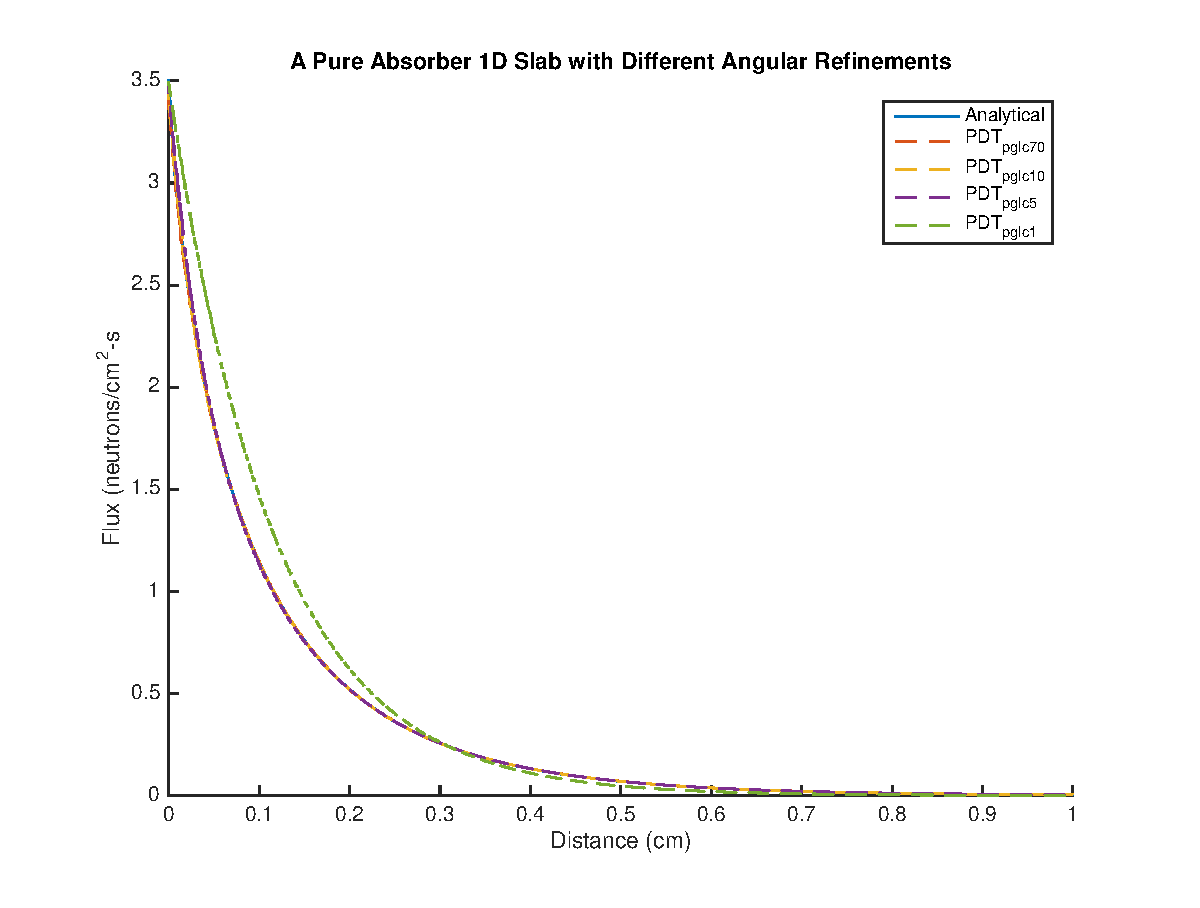
\includegraphics[scale = 0.8]{figures/PureAbsorberAllAngles.eps}
\captionof{figure}{The pure absorber solution with four different angular refinements.}
\label{pa_allangles}
\end{minipage}
\smallskip

It is immediately clear that not many polar angles are necessary for agreement with the analytical solution. Figure \ref{pa_bestangle} examines the 70 positive polar angle case exclusively in comparison with the analytical solution. It is immediately clear graphically that the solutions are in agreement. Table \ref{flux_errors} shows the error convergence as the number of cells in the problem increases.

\noindent\begin{minipage}{\textwidth}
\centering
\includegraphics[scale = 0.8]{figures/PureAbsorberBestangle.eps}
\captionof{figure}{The pure absorber solution run with 70 positive polar angles.}
\label{pa_bestangle}
\end{minipage}
\smallskip

\begin{table}[H]
\centering
\caption{The convergence of the error as the number of cells increases.}
\begin{tabular}{c c}
\hline
\textbf{Number of Cells} & \textbf{$\epsilon$} \\
8 & 0.3035 \\
32 & 0.1865 \\
128 & 0.09168 \\
512 & 0.0387 \\
\hline
\end{tabular}
\label{flux_errors}
\end{table}
\smallskip

\subsection{The 1D Pure Scatterer Slab}

For an optically thick, source free 1D pure absorber with monoenergetic neutrons, the transport solution will reach the diffusion limit. The diffusion equation for this problem is represented by Eq. ~\eqref{diffusion}:
%Scattering equation
\begin{equation}
\frac{d^2\phi}{dx^2} = 0,
\label{diffusion}
\end{equation}
where $\phi$ is the scalar flux. The boundary conditions for this problem are expressed in Eq. ~\eqref{scatterboundary}:
%Scatter bc's
\begin{align}
\phi(-2D) &= 4j_{inc} \notag \\
\phi(x_{\text{max}}+2D) &= 0, 
\label{scatterboundary}
\end{align}
where $j_{inc}$ is the incident partial current and $D$ is the diffusion coefficient, which is equivalent to $\frac{1}{3 \Sigma_t}$, where $\Sigma_t$ is the total macroscopic cross section. The first boundary condition is the extrapolated boundary condition, and the second is the extrapolated vacuum condition. The incident partial current is calculated from the incident angular flux, as shown in Eq. ~\eqref{partialcurrent}:
%Partial current
\begin{equation}
j_{inc} = \int_{0}^{2\pi}d\gamma \int_{0}^{1} \mu \frac{\psi_{inc}}{4\pi} d\mu = \frac{\psi_{inc}}{4}.
\label{partialcurrent}
\end{equation}

The integral over polar angles in Eq. ~\eqref{partialcurrent} is the result of computing the angular quadrature with an infinite number of polar angles. Table \ref{angleconvergence} shows the value of $j_{inc}$ converging to the integral value as the number of polar angles is increased. 
\begin{table}[H]
\centering
\caption{The convergence of $j_{inc}$ as the number of polar angles increase.}
\begin{tabular}{c c}
\hline
\textbf{Number of Positive Polar Angles} & \textbf{$j_{inc}$} \\
1 & 2.0207 \\
2 & 1.8244 \\
5 & 1.7632 \\
10 & 1.7534 \\
20 & 1.7509 \\
40 & 1.7502 \\
Infinite & 1.750 \\
\hline
\end{tabular}
\label{angleconvergence}
\end{table}

Equation ~\eqref{scalarflux} solves Eq. ~\eqref{diffusion}:
\begin{align}
\frac{d\phi(x)}{dx} &= A \notag \\
\phi(x) &= Ax + B,
\label{scalarflux}
\end{align}
where A and B are integration constants. Using our boundary conditions in Eq ~\eqref{scatterboundary} to solve for A and B:
\begin{align}
\phi(-2D) &= -2DA + B = 4j_{inc} \notag \\
\phi(x_{\text{max}} + 2D) &= A(x_{\text{max}} + 2D) + B = 0, \notag
\label{notimportant}
\end{align}
the scalar flux, represented by Eq. ~\eqref{scatterflux}, is:
%Scatter flux
\begin{equation}
\phi(x) = \frac{4j_{inc}}{1+4D}(-x + x_{\text{max}} + 2D).
\label{scatterflux}
\end{equation}

This problem was run with $\Sigma_t = 100 \text{ cm}^{-1}$ and $j_{inc} = \frac{7}{4} \frac{\text{n}}{\text{cm}^2\text{-s}}$. Figure \ref{scattersoln} shows the agreement between the analytical solution and PDT's solution. An angular refinement of 40 polar angles was used, with one azimuthal angle in each quadrant.

\noindent\begin{minipage}{\textwidth}
\centering
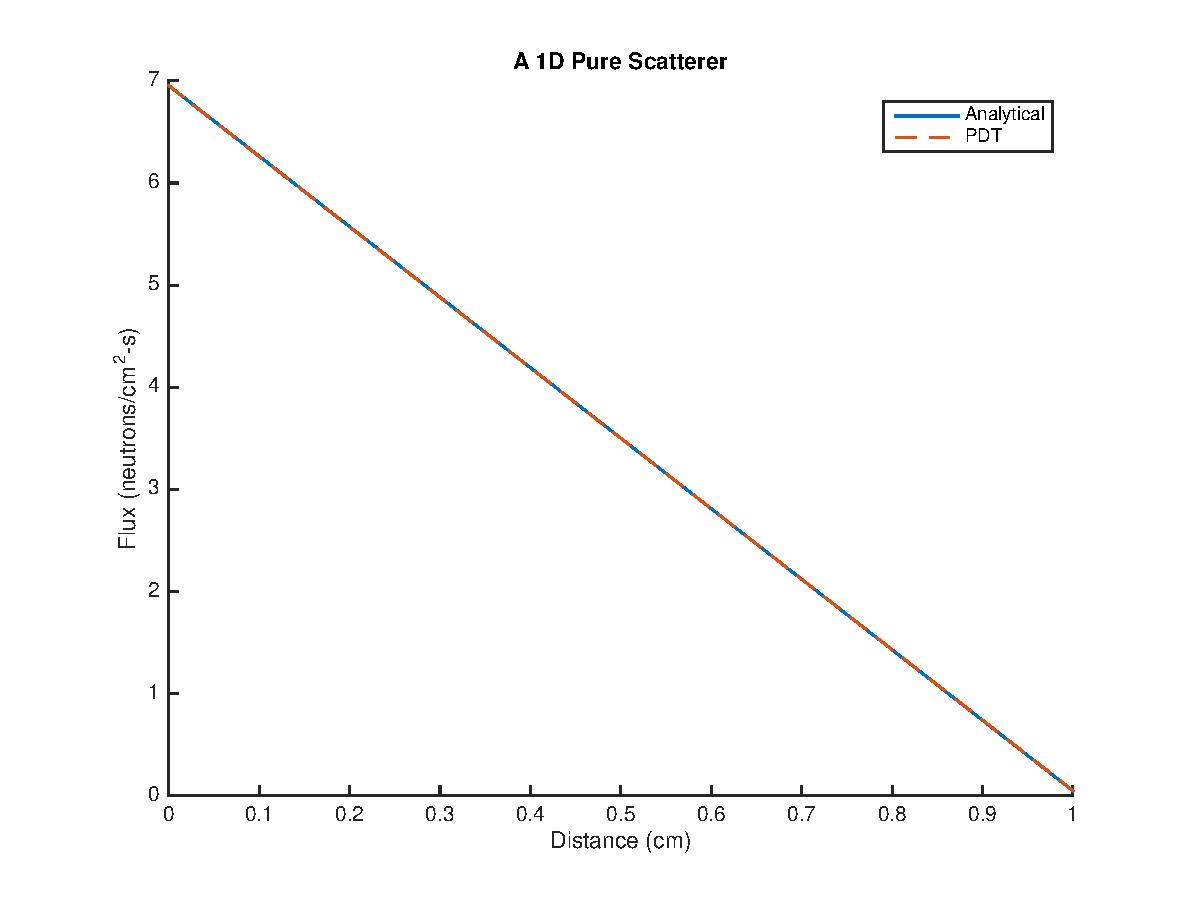
\includegraphics[scale = 0.8]{figures/PureScatterer.eps}
\captionof{figure}{The pure scatterer solution run with 40 positive polar angles.}
\label{scattersoln}
\end{minipage}
\smallskip

It is immediately clear graphically that the two solutions are in agreement, and the relative error of the numerical solution is 4.25E-04, as defined by Eq. ~\eqref{error}.

\section{2D and 2D Extruded Meshing Capability}

To showcase, the newly implemented unstructured meshing capability in PDT, Texas A\&M Nuclear Engineering's Impurity Model 1 (IM1) problem is used. Figure \ref{IM12D} showcases the 2D mesh of the IM1 problem,

\noindent\begin{minipage}{\textwidth}
\centering
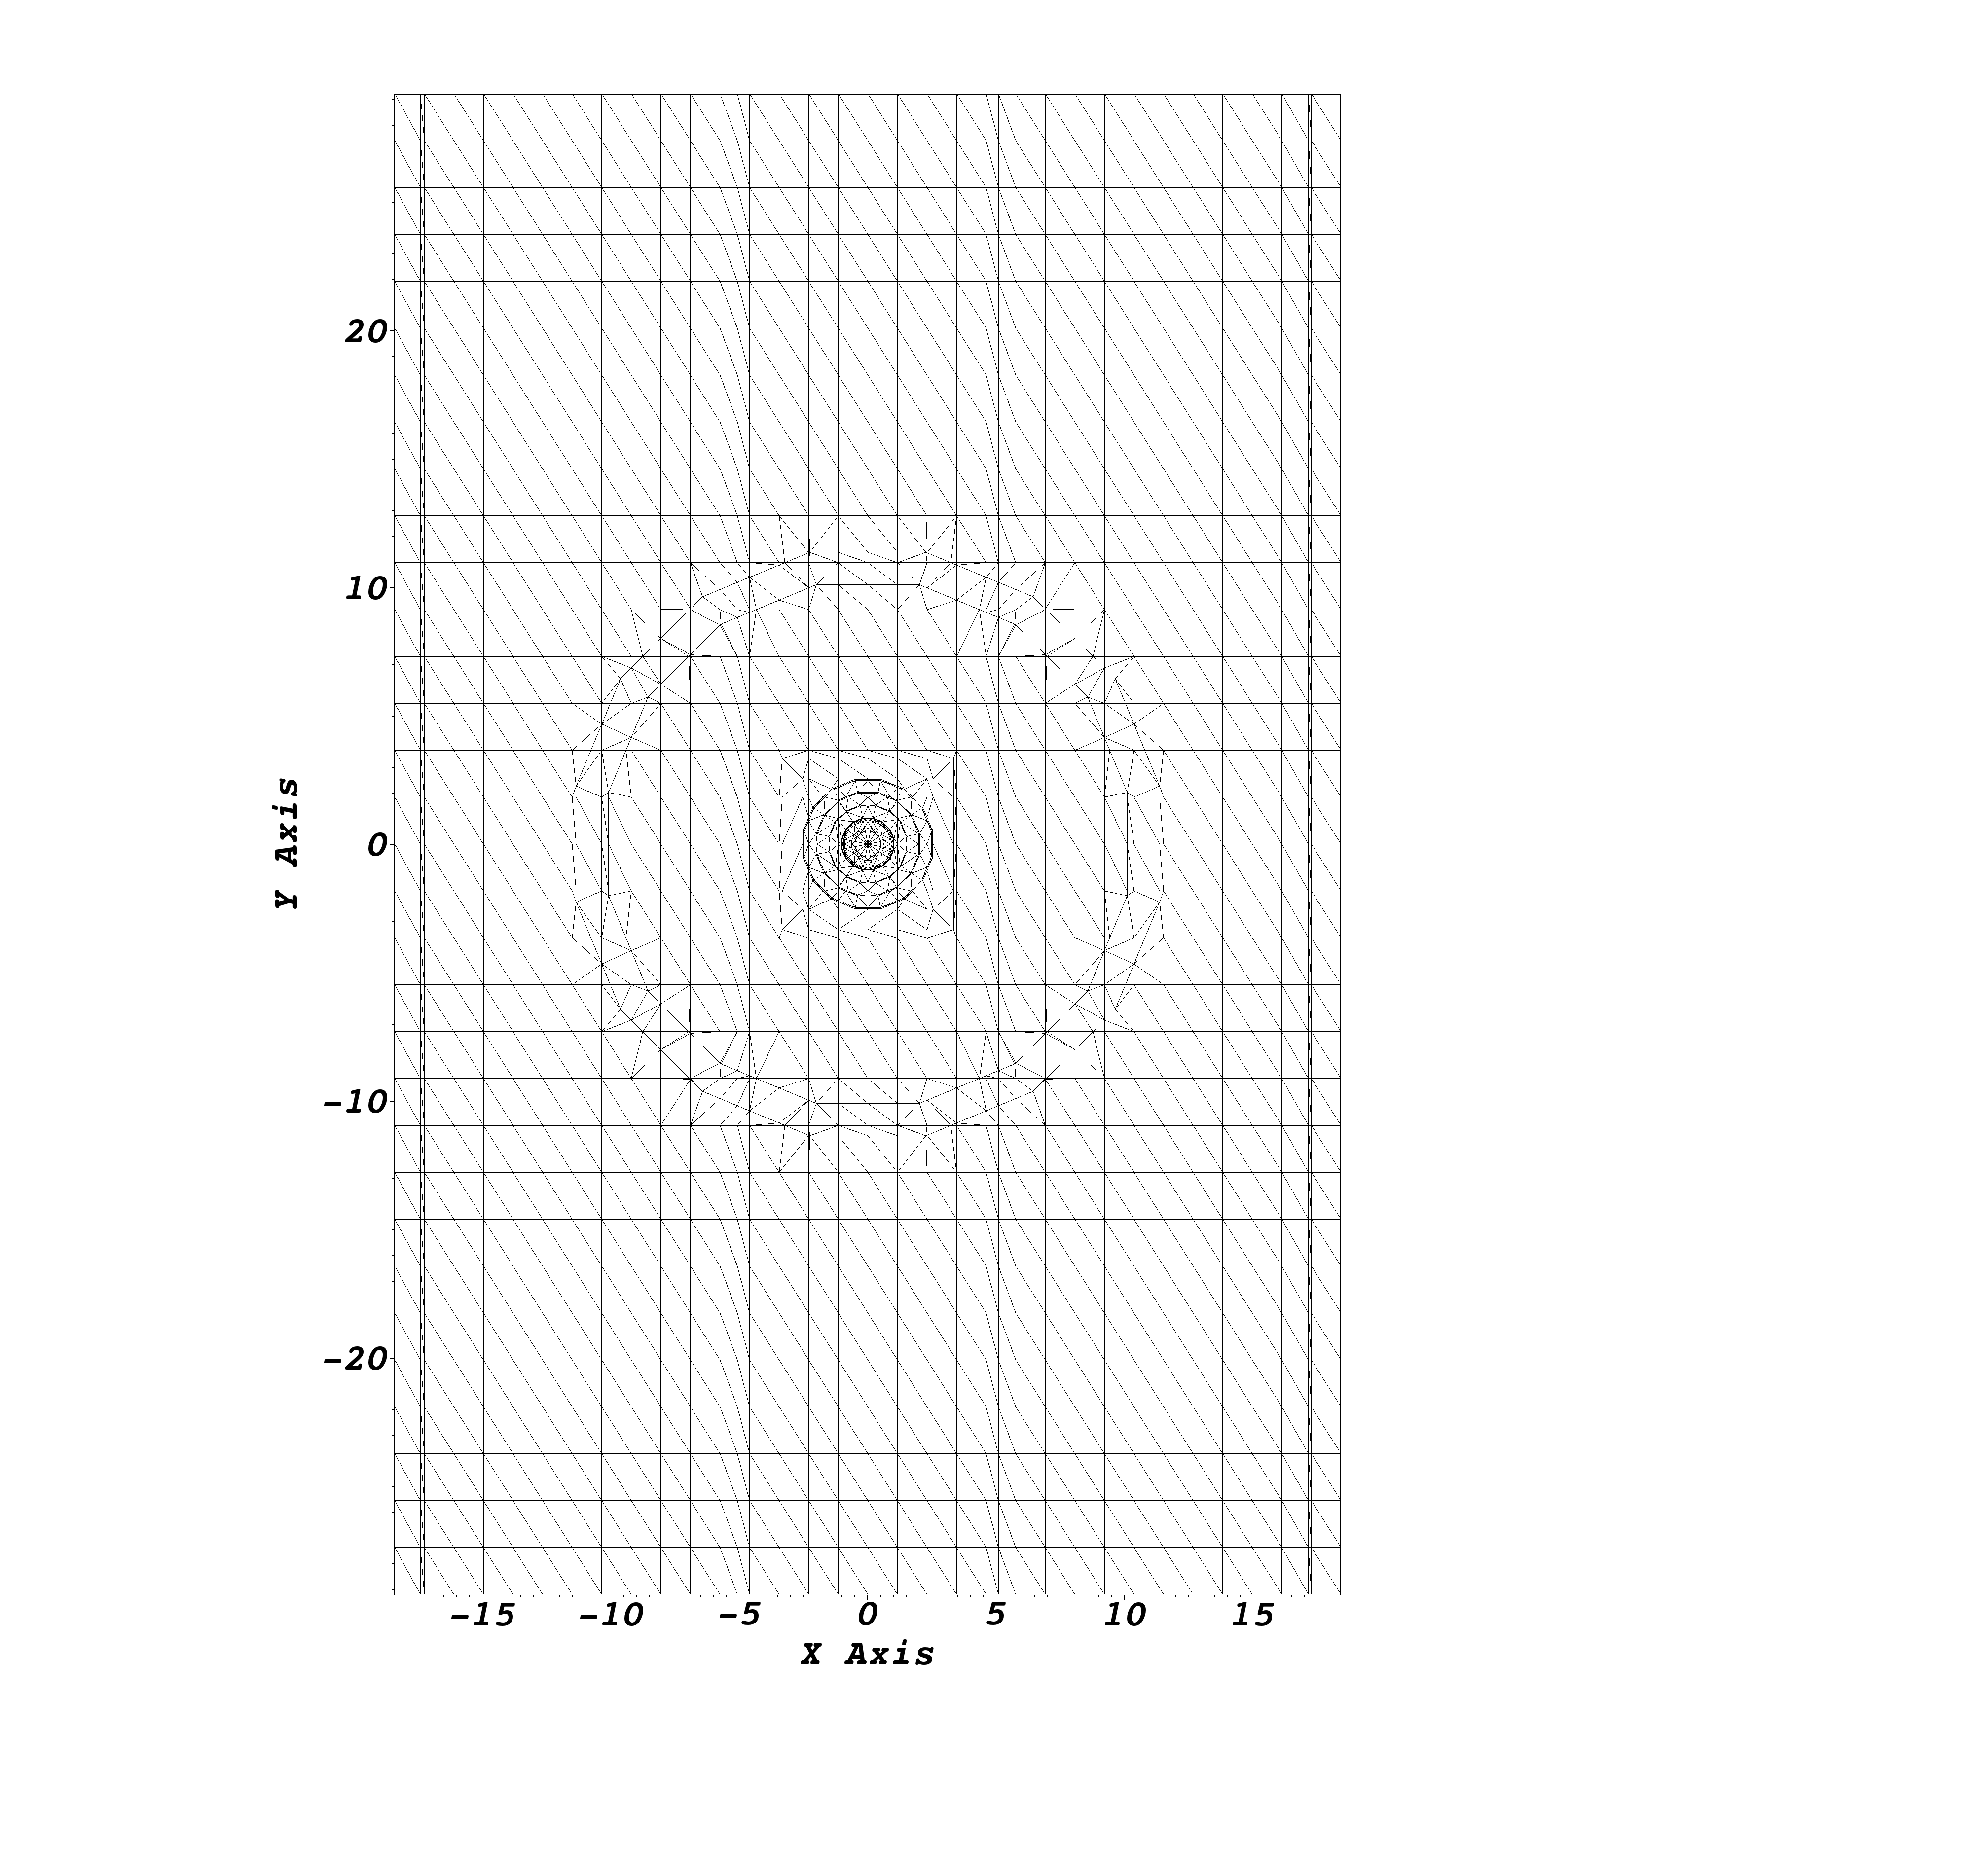
\includegraphics[scale = 0.13]{figures/im12d.png}
\captionof{figure}{The 2D mesh of the IM1 problem.}
\label{IM12D}
\end{minipage}
\smallskip

In order to get from the 2D mesh to the 2D extruded mesh, an extrusion file is supplied to PDT. This extrusion file supplies two critical pieces of information: the number of z layers and their locations, and how each region of the 2D mesh is mapped to these z layers. The combination of the 2D mesh and the extrusion file yield the full 3D problem, shown in Fig. \ref{IM13D}.

\noindent\begin{minipage}{\textwidth}
\centering
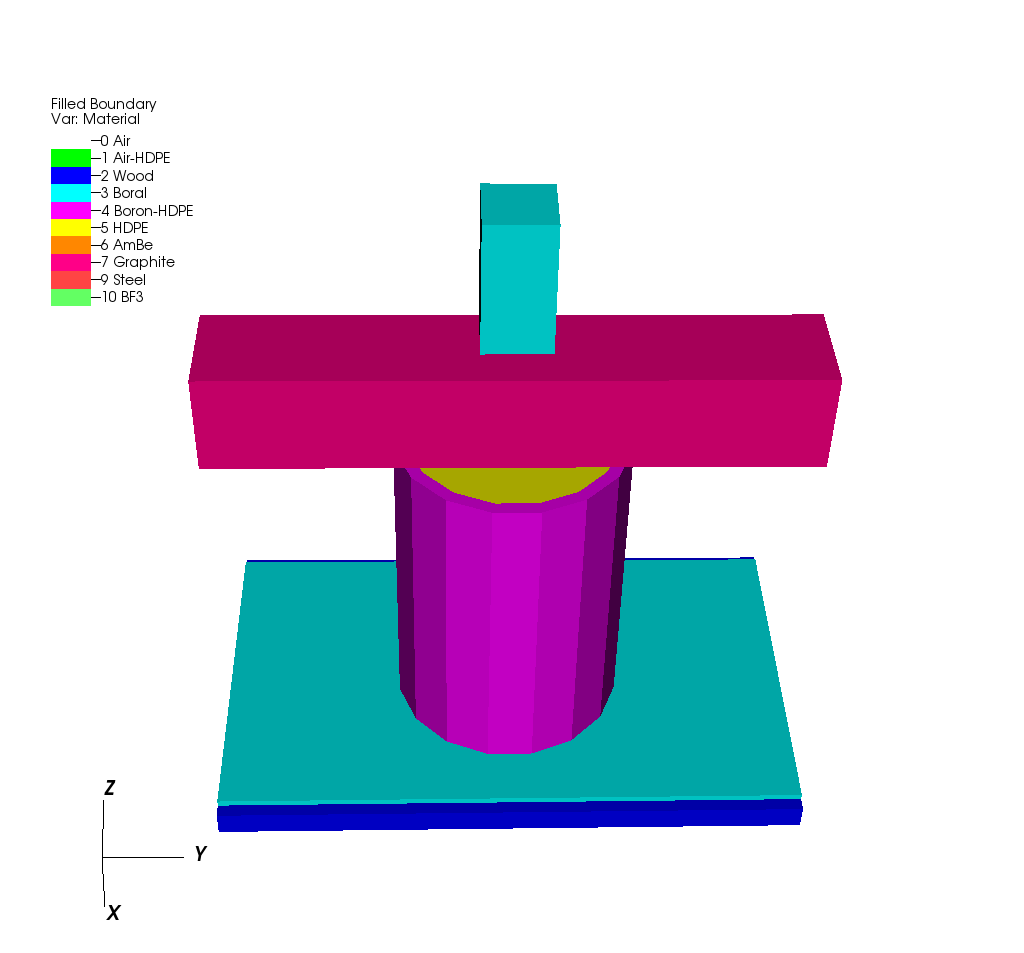
\includegraphics[scale = 0.5]{figures/IM1_3D.png}
\captionof{figure}{The 2D extruded view of the IM1 problem.}
\label{IM13D}
\end{minipage}
\smallskip

%\noindent\begin{minipage}{\textwidth}
%\centering
%\hspace*{-3 cm}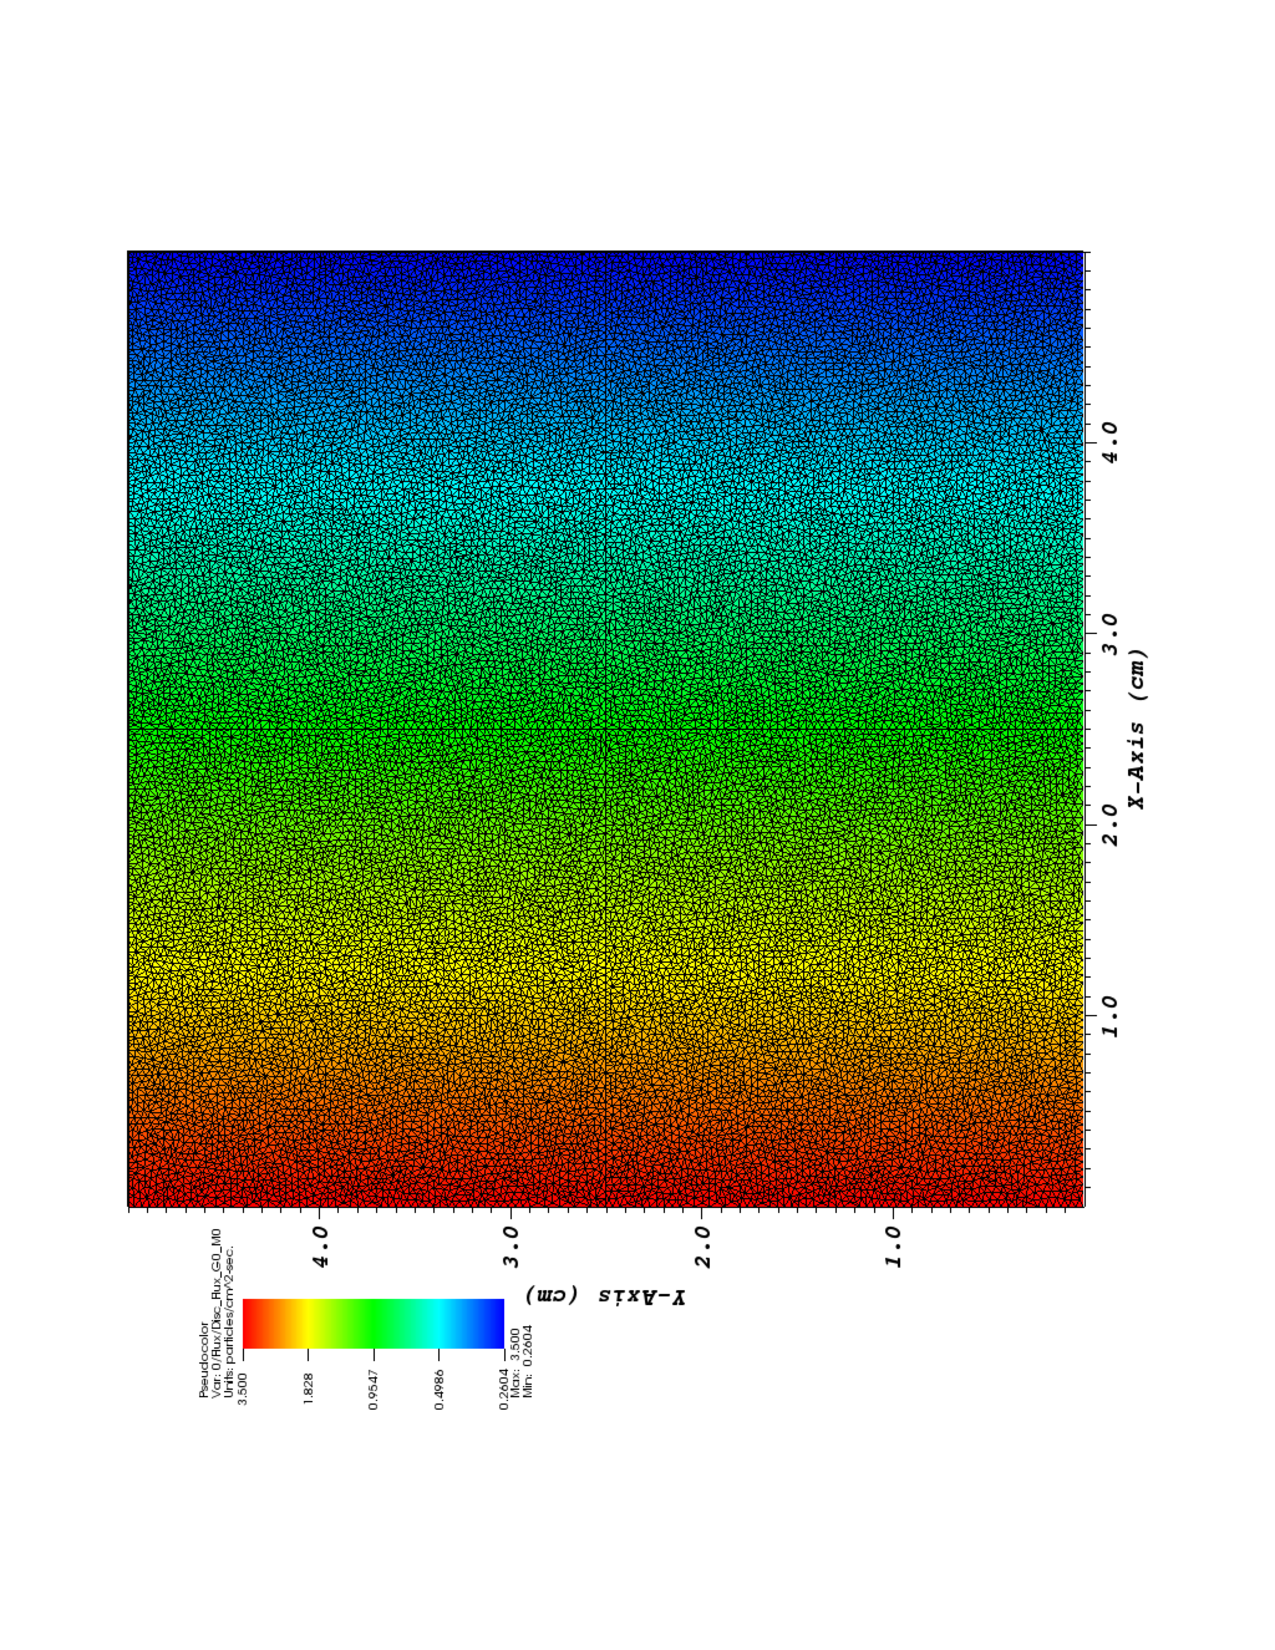
\includegraphics[scale=0.8,angle=-90]{figures/PureAbsorberSolution.pdf}
%\captionof{figure}{The solution of a pure absorbing slab.}
%\label{pureabsorber}
%\end{minipage}
